%%
%% Copyright 2007, 2008, 2009 Elsevier Ltd
%%
%% This file is part of the 'Elsarticle Bundle'.
%% ---------------------------------------------
%%
%% It may be distributed under the conditions of the LaTeX Project Public
%% License, either version 1.2 of this license or (at your option) any
%% later version.  The latest version of this license is in
%%    http://www.latex-project.org/lppl.txt
%% and version 1.2 or later is part of all distributions of LaTeX
%% version 1999/12/01 or later c.
%%
%% The list of all files belonging to the 'Elsarticle Bundle' is
%% given in the file `manifest.txt'.
%%

%% Template article for Elsevier's document class `elsarticle'
%% with harvard style bibliographic references
%% SP 2008/03/01
%%
%%
%%
%% $Id: elsarticle-template-harv.tex 4 2009-10-24 08:22:58Z rishi $
%%
%%
\documentclass[preprint,authoryear,12pt]{elsarticle}

%% Use the option review to obtain double line spacing
%% \documentclass[authoryear,preprint,review,12pt]{elsarticle}

%% Use the options 1p,twocolumn; 3p; 3p,twocolumn; 5p; or 5p,twocolumn
%% for a journal layout:
%% \documentclass[final,authoryear,1p,times]{elsarticle}
%% \documentclass[final,authoryear,1p,times,twocolumn]{elsarticle}
%% \documentclass[final,authoryear,3p,times]{elsarticle}
%% \documentclass[final,authoryear,3p,times,twocolumn]{elsarticle}
%% \documentclass[final,authoryear,5p,times]{elsarticle}
%% \documentclass[final,authoryear,5p,times,twocolumn]{elsarticle}

%% if you use PostScript figures in your article
%% use the graphics package for simple commands
%% \usepackage{graphics}
%\usepackage{cases}
%% or use the graphicx package for more complicated commands
\usepackage{graphicx}
%% or use the epsfig package if you prefer to use the old commands
\usepackage{epsfig}

\usepackage{comment}
\usepackage{epstopdf}
\usepackage{bm}
\usepackage{hyperref}
\hypersetup{colorlinks=true, urlcolor=blue, linkcolor=blue, citecolor=red}

%% The amssymb package provides various useful mathematical symbols
\usepackage{amssymb,amsmath}
%% The amsthm package provides extended theorem environments
%% \usepackage{amsthm}

%% The lineno packages adds line numbers. Start line numbering with
%% \begin{linenumbers}, end it with \end{linenumbers}. Or switch it on
%% for the whole article with \linenumbers after \end{frontmatter}.
%% \usepackage{lineno}

%% natbib.sty is loaded by default. However, natbib options can be
%% provided with \biboptions{...} command. Following options are
%% valid:

%%   round  -  round parentheses are used (default)
%%   square -  square brackets are used   [option]
%%   curly  -  curly braces are used      {option}
%%   angle  -  angle brackets are used    <option>
%%   semicolon  -  multiple citations separated by semi-colon (default)
%%   colon  - same as semicolon, an earlier confusion
%%   comma  -  separated by comma
%%   authoryear - selects author-year citations (default)
%%   numbers-  selects numerical citations
%%   super  -  numerical citations as superscripts
%%   sort   -  sorts multiple citations according to order in ref. list
%%   sort&compress   -  like sort, but also compresses numerical citations
%%   compress - compresses without sorting
%%   longnamesfirst  -  makes first citation full author list
%%
%% \biboptions{longnamesfirst,comma}

% \biboptions{}
\newcommand{\PN}[2][error]{P$_{#1}$DG-P$_{#2}$}


\journal{Computer Methods in Applied Mechanics and Engineering}

\begin{document}

\begin{frontmatter}

%% Title, authors and addresses

%% use the tnoteref command within \title for footnotes;
%% use the tnotetext command for the associated footnote;
%% use the fnref command within \author or \address for footnotes;
%% use the fntext command for the associated footnote;
%% use the corref command within \author for corresponding author footnotes;
%% use the cortext command for the associated footnote;
%% use the ead command for the email address,
%% and the form \ead[url] for the home page:
%%
%% \title{Title\tnoteref{label1}}
%% \tnotetext[label1]{}
%% \author{Name\corref{cor1}\fnref{label2}}
%% \ead{email address}
%% \ead[url]{home page}
%% \fntext[label2]{}
%% \cortext[cor1]{}
%% \address{Address\fnref{label3}}
%% \fntext[label3]{}

\title{The Overlapping Control Volume Finite Element Method for Multi-Fluids Porous Media Flow Modelling. Part II: Simulation Results}

\author[IC]{D. Pavlidis}\corref{cor1}\ead{dimitrios.pavlidis@imperial.ac.uk} \author[UoA]{J.L.M.A. Gomes}  \author[IC]{J.R. Percival} \author[IC]{P. Mostaghimi} \author[IC]{P. Salinas} \author[IC]{Z. Xie} \author[IC]{C.C. Pain} \author[IC]{M. D. Jackson} \author[HW]{A.H. ElSheikh} \author[IC]{M. Blunt} \author[IC]{A. Muggeridge}  
\cortext[cor1]{Corresponding author.}

\address[IC]{Applied Modelling and Computation Group, Department of Earth Science and Engineering, Imperial College London, UK}
\address[UoA]{Environmental $\&$ Industrial Fluids Mechanics Group, School of Engineering, University of Aberdeen, UK}
\address[HW]{Institute of Petroleum Engineering, Heriot-Watt University, Edinburgh, UK}


\begin{abstract} 
This paper is the second in a series of manuscripts on novel FEM-based formulations for multi-scale compositional multi-fluid porous media flows. In the first paper, the multiphase formulation, based upon the overlapping control volume discontinuous-Galerkin finite element method (OCV-DGFEM), was fully described and, advection-diffusion validation test-cases were used to demonstrate the accuracy and convergence of the formulation. In this second paper, the OCV-DGFEM-based formulation is applied to a set of multi-fluids porous media flows test-cases to assess the performance and numerical accuracy of (a) element-pairs (\PN[n]{n+1}, \PN[n]{n+1}DG, \PN[n]{n} and \PN[n]{n}DG), (b) continuous / discontinuous (between elements) formulations, (c) structured and unstructured (triangle / tetrahedron) meshes, (d) upwind schemes and (e) domain heterogeneities imposed by large permeability ratios. Numerical solutions are in good agreement with (semi-)analytically and experimentally obtained data.
\end{abstract}

\begin{keyword}
%% keywords here, in the form: keyword \sep keyword
Multiphase porous media flow \sep DG methods \sep Mixed FEM formulation \sep Permeability discretisation \sep Computational multi-fluids dynamics. 
\end{keyword}

\end{frontmatter}

%\tableofcontents
% \linenumbers
%%%                   %%%
%%%      SECTION      %%%
%%%                   %%%
\section{Introduction}

\begin{itemize}
\item \textcolor{red}{One relatively short paragraph on main motivation for the work.}
\end{itemize}

In recent years, advances in numerical simulation techniques have played an increasing role in solving complex engineering problems. Most of these problems can be represented as fully coupled systems of nonlinear partial differential equations in a multitude of spatial- and temporal-scales. Novel mathematical methods have been continuously introduced to improve both numerical accuracy and convergence of equations' solutions while also aiming for optimum computational performance. 

Finite difference methods (FDM) still are the preferred numerical tool for subsurface flows in industrial-standard models due to the inherent simplicity and ease of implementation. However FDM-based models often lack geometry flexibility and numerical accuracy and therefore have been mostly restricted to aged software packages.  Due to the simple physical interpretation, numerical accuracy $\&$ robustness and elegant mathematical formulation, finite element and volume methods (FEM and FVM) have attracted the attention of scientists and engineers interested in multi-physics applications in complex geometries \citep{cordazzo_2006, geiger_2004,nick_2011}. 

Among the different families of finite element methods, mixed FEM gained great attention due to (a) high accuracy of field solutions and associated fluxes, (b) boundedness of solution (essential to physical realism) and (c) local mass conservation \citep[within an element,][]{fung_1992,durlofsky_1993,durlofsky_1994}. However, they are often plagued by very expensive computational overhead in shock-dominated conditions, e.g., large permeability ratios in fractured porous media interfaces. Discontinuous Galerkin (DG) method is another family of FEM that utilises discontinuous piecewise polynomial spaces and specialised bi-linear forms to weakly impose boundary conditions and inter-element connectivities.  DGFEM methods became popular in scientific computing communities as they are able to ensure local mass conservation with relatively small numerical diffusion and solution's oscillations whilst support nonconforming unstructured tetrahedral meshes and {\it h-p} adaptive methods \citep{merton_2012,brooks_1982}. 




This is the second of a series of papers exploiting novel computational methods for multi-fluids flow in porous media. The new overlapping control volume finite element method was introduced in the first part of this series followed by an advection test-case validation \citep{gomes_2013}. The formulation lies in two-folds development, it uses a dual consistent pressure-velocity representation in CV and DGFEM spaces (through a mixing formulation) and a recently developed \PN[n]{n+1} family of FE types. Additionally a novel family of fully discontinuous element types -- the \PN[n]{n+1}DG and \PN[n]{n}DG, was introduced to represent discontinuity across neighbour elements able to represent highly heterogeneous porous media domain, typical of some geological formations.

The remainder of this paper is organised as follows. A brief description of the model is given in Section~\ref{Section:SummaryPaper1} followed by the model validation against analytical solutions of the classical Buckley-Levrett problem. In Section~\ref{res2}, water-flood problems (i.e., immiscible fluids displacement) were simulated in 2-D geometry to assess the flow behaviour in prescribed heterogeneous porous media. The impact of large permeability ratios (i.e., highly heterogeneous porous matrix) in the model was investigated in Sections~\ref{res3} and~\ref{res4}. Additionally, in the later we also investigated the model performance when elements are skewed due to large domain aspect ratio. A brief summary of the results are presented in Section~\ref{conc} followed by many conclusions drawn from the two inter-linked papers. 



%\setlength\parindent{0pt}


%\section{Model Validation}\label{Section:Results}
\section{Summary of the Model Formulation}\label{Section:SummaryPaper1}
This section summarises the model formulation to solve multiphase porous media equations.  The novel overlapping control volume - discontinuous Galerkin finite element method (OCV-DGFEM) is based on two-fold numerical development, a FEM-based mixed formulation and a new family of element-pairs (\PN[n]{n+1}).  The underlying mass balance equations (e.g., saturation, density, mass fraction, etc.) are solved in control volume (CV) space whereas a Petrov-Galerkin FEM is used to obtain the high-order fluxes on the CV boundaries which are limited to achieve bounded mass-based fields (e.g., positiveness of densities and saturations ranging from zero to one).

The family of \PN[n]{n+1} element-pairs was introduced by \citet{cotter_2009b} \citep[see also][]{cotter_2011} for geophysical fluid dynamics (GFD) applications. In particular, \PN[1]{2} elements -- linear discontinuous polynomial FE basis function for velocity $\left(\text{P}_{1}\text{DG}\right)$ and quadratic polynomial FE basis function for pressure $\left(\text{P}_{2}\right)$, was developed to represent the balance of geostrophic pressure and velocity without introducing spurious pressure modes. Any numerical discretisation that is not based upon quadrilaterals and hexahedra mesh grids very often results in spurious pressure modes due to the unbalancing number of velocity and pressure degrees-of-freedom \citep{sollie_phd_2010}.  However, tests on the \PN[1]{2} element-pair proved that this element is LBB stable \citep{cotter_2009a} and does not present spurious pressure modes on arbitrary unstructured meshes. 

The extended Darcy's law for $N_{p}$ immiscible fluid phases can be expressed as
\begin{equation}
S_{k}\left(\displaystyle\frac{\mathbf{K} \mathcal{K}_{rk}}{\mu_{k}}\right)^{-1}\mathbf{u}_{k}=\underline{\underline{\sigma}}_{k} \mathbf{u}_{k} = -\nabla p + \mathbf{s}_{u} 
\end{equation}
where $k\in\left[1,N_{p}\right]$ represents the phase, $S$, $\mathbf{K}$, $\mathcal{K}_{r}$ and $\mu$ are saturation, permeability tensor, relative permeability and viscosity, respectively. $\mathbf{u}$, $\mathbf{s}_{u}$ and $p$ are the saturation-weighted Darcy velocity, a source-like term (e.g., gravity forces) associated with the force balance and the pressure.  

$\underline{\underline{\sigma}}_{k}$ is an absorption-like term with coupled FE and CV representation of the nonlinear convolution of saturation, relative permeabilities, porosity and permeability tensor fields. This term, representing the viscous frictional forces, is piecewise constant within each FE and is obtained via basis functions local to each CV within each element. An overlapping (or hybrid) basis functions formulation were introduced in \citet{gomes_2013} assuming that there is a (nonlinear) functional that correlates velocity with a FE and the corresponding CVs velocity components basis functions,
\begin{eqnarray} 
 %\sum\limits_{E}\int_{\Omega_E} { {Q}}_i \left({\underline {\underline \sigma}}_k \cdot  {\mathbf u} + \nabla p -{\mathbf s}_u \right) dV +  \displaystyle\frac{1}{2} \oint_{\Gamma_{E}}  {Q}_i {\mathbf n} \left(p - p_{nab}\right) d\Gamma + \nonumber \\
 \sum\limits_{E} \left. \int\limits_{\Omega_E} { {Q}}_i \left({\underline {\underline \sigma}}_k  {\mathbf u} + \nabla p -{\mathbf s}_u \right) dV \right. +  \displaystyle\frac{1}{2} \oint_{\Gamma_{E}}  {Q}_i {\mathbf n} \left(p - p_{nab}\right) d\Gamma + \nonumber \\
 \oint_{\Gamma_{\Omega}} { Q}_i {\mathbf n} \left(p - p_{bc}\right) d\Gamma = \bm{0}
\label{force-semi-disc} 
\end{eqnarray} 
with
\begin{displaymath}
p = \sum\limits_{j=1}^{\mathcal{N}_p} P_{j}p_{j} \;\;\;\;\text{  and  }\;\;\;\; u_k=\sum\limits_{j=1}^{\mathcal{N}_u} Q_{j}u_{k,j}.
\end{displaymath} 
in which $\mathcal{N}_{p}$ and $\mathcal{N}_{u}$ are the number of degrees of freedom for the FE pressure and velocity representations, respectively. $\Omega_E$ is the volume domain of element $E$ associated with the FE velocity, $\Gamma_{E}$ is the surface boundary of $E$ and $\Gamma_{\Omega}$ is the boundary of the entire domain. $p_{nab}$ is the pressure value on the other side of the element boundary neighbouring element $E$.
Phase-saturation equations,
\begin{equation}\label{Eqn:Saturation}
  \phi\displaystyle\frac{\partial \rho_{k} S_{k} }{\partial t}  + \nabla \cdot \left( {\mathbf u}_{k} \rho_{k} S_{k}\right) = s_{cty,k} 
\end{equation}
are discretised in space by testing with CV basis functions and in time with the $\theta$-method,
\begin{eqnarray}
&&
\sum\limits_{k}^{\mathcal{N}_{p}} 
\left\{  
\int_{\Omega} M_{i} \left[  
\displaystyle\frac{ {S_{k}}_{i}^{n} {\nu_{k,i}^{n+1}} \left( {p_{CV}}_{i}^{n+1} - \tilde{p_{CV}}_i^{n+1} \right)} { {\rho_{k}}_{i}^{n} \Delta t } + \displaystyle\frac{ {S_{k}}_{i}^{n} \left( \tilde{ {\rho}_{k}}_{i}^{n+1} - {\rho_{k}}_{i}^{n} \right) } { { \rho_{k}}_{i}^{n} \Delta t }
\right] dV \right. \nonumber \\
&&
\left. 
 + \displaystyle\frac{1}{ {\rho_{k}}_{i}^{n} } \oint_{ {\Gamma_{CV}}_{i}} \mathbf{n} \cdot \mathbf{u}_{k}^{n+\theta} \rho_{k}^{n+\theta} S_{k}^{n+\theta} d\Gamma -\displaystyle\frac{1}{ {\rho_{k}}_{i}^{n} } \int_{\Omega} M_{i} s_{cty,k}^{n+\theta} dV
\right\} = 0,
  \label{detail-global-cty}
\end{eqnarray}
In Eqn. \ref{Eqn:Saturation}, $\phi$, $\rho$ and $s_{cty}$ are the rock-matrix porosity, fluid density and source-like term associated with the global continuity equation. $\nu$ represents the CV-based projection fluids compressibility. Pressure matrix equation is produced by summing the CV-based discretised global mass balance and the overlapping CV-DGFEM-based discretised Darcy equations. At time level $n+1$, the coupled multiphase Darcy and global mass conservation are represented, in matricial form, as
\begin{equation}
\begin{cases}
\mathbf{M}_{\sigma} \underline{\bf u}^{n+1} = \mathbf{C}\underline{\bf p}^{n+1} + \underline{\bf s}_{u}^{n+1} \\
\mathbf{M}_{p} \underline{\bf p}^{n+1} + \mathbf{B}^{T} \underline{\bf u}^{n+1} = \underline{\bf s}_{p}^{n+1}
\end{cases}
\end{equation}

\section{Classical Buckley-Leverett Test-Cases}\label{classical_BL}
The Buckley-Leverett equation \citep[B-L,][]{doster_2011,proskurowski_1981} is commonly used in petroleum industry to represent the displacement of fluids in porous media for oil recovery. When oil is initially produced, the pressure is sufficiently high to force the flow of the oil and gas through the producing wells. However, the rate in which oil is produced drops with time as the pressure naturally decreases. In order to keep the production rate, fluids $\left(\text{e.g., supercritical CO}_{2}\text{ and/or water}\right)$ are injected to drive the oil towards production wells. The B-L equation is a nonlinear advection equation for the relative saturation of fluid phases representing two-phase immiscible flows in porous matrix. 

In this section, incompressible two-phase displacements is simulated with water $\left(S_{l}=1\right)$ being injected at a velocity $u_{1}=1$ into a fully saturated porous matrix containing non-wetting and immobile oil $\left(S_{2}=1,\;\phi=0.5\right)$. For relative permeability calculations $\left(\mathcal{K}_{rk}\right)$, the irreducible and residual water saturations are set to 0.2 and 0.1, respectively. The length of the domain is 4 non-dimensional units, the endpoint of oil and water relative permeabilities are 0.3 and 0.8, while Corey exponent is assumed as 2. On the outlet boundary condition, the pressure level is set to zero and all remaining boundary conditions are weakly applied. 

Despite the one-dimensional nature of the problem, 2- and 3-D simulations were performed using structured and unstructured meshes to evaluate the multi-dimensional capabilities of the model. In 2- and 3-D simulations, free-slip boundary conditions are applied on the sides of the domain for the two velocity fields.

 All simulations used the overlapping mixed-DGFEM with \PN[0]{1}, \PN[1]{2} and/or \PN[2]{3} element-pairs with continuous / discontinuous (between elements) formulations with saturation collocated at pressure nodes. Although saturation is calculated using a CV formulation, a FEM interpolation is used to form the high-order fluxes and these are also used for most of the plots. In all 1-D simulations, mesh grids were designed with equi-sized elements, whilst 2-D meshes were regular, structured and one-element wide with unity aspect ratio. The width of the 2-D numerical domain is inversely proportional to the number of elements. The time-step size varied linearly within 0.125-3.125$\times$10$^{-3}$ seconds range for 1-D simulations, and 1.0$\times$10$^{-4}$ for all 2- and 3-D simulations.

\subsection{Continuous Formulation}
\paragraph{Upwind Solution} 
In Fig.~\ref{bl-exact-meth-upwind} the CV solution of the water-phase saturation and equivalent quadratic FEM interpolation are presented (\PN[1]{2}). As it can be seen, the solution converges with increased resolution. Notice that the corners of the CVs are very close to the converged solution. This can be explained as the velocities are upwinded (and also the relative permeabilities), and at these corners the equations reach the balance necessary to match the analytical solution.

\paragraph{Convergence Analysis}
Convergence analysis were performed for the 1- and 2-D problems with a number of (regular) mesh resolution and element pairs. The time-step size was linearly varied from 1.25$\times$10$^{-4}$ to 3.25$\times$10$^{-3}$ seconds. Figure~\ref{fig:BL_profiles} shows water-phase saturation profiles at time $t=0.5$ for mesh grids varying from 5 to 500 elements, and for different element types -- \PN[0]{1}, \PN[1]{2} and \PN[2]{3} (the geometry symmetry line is used to extract data from the 2-D simulations).  In general, results are in good agreement with the analytic solution for all resolutions and element-pairs however, for coarser meshes, high-order elements-pairs (\PN[2]{3} for 1-D using 5 elements and \PN[1]{2} for 2-D using 20 elements) perform significantly better and are able to capture the sharp-front more accurately. As far as the 2-D simulations are concerned, the coarse mesh simulation performs slightly worse than its 1-D counterpart but for higher resolutions, results are identical.

These conclusions become clearer in Fig.~\ref{fig:BL_converg-rates}, where convergence rates are shown. The L1 and L2 errors are defined as,
\begin{displaymath}
\displaystyle\frac{\sum\limits_{i=1}^{N}\left|S_{i}^{\text{simulated}}-S_{i}^{\text{analytical}}\right|}{N}\;\;\text{ and }\;\; \displaystyle\frac{\sum\limits_{i=1}^{N}\sqrt{\left(S_{i}^{\text{simulated}}-S_{i}^{\text{analytical}}\right)^{2}}}{N},
\end{displaymath}
respectively, where $S$ is the water-phase saturation. In addition, convergence rates for simulations performed with full upwinding scheme are also shown.


\paragraph{Optimal Upwinding} 
%In order to optimise the upwind formulation (Section~\ref{FluxLimitingSection}), we investigated a 80/20$\%$ up/downwinding ratio -- Fig.~\ref{bl-exact-meth-cv-0-8-ele50}, with good agreement with the converged solution. 
An appropriate upwind fraction may lead to the  increase of accuracy of the formulation -- here the fraction was varied from 1 (full upwinding -- typically applied near shock-fronts) to $\frac{1}{2}$ (i.e., central differencing scheme).  However, even though downwind scheme (for the velocity field) may also help increasing the accuracy we limit the current scheme to central difference. If however, a coupled up/downwind scheme (80/20$\%$ ratio) is chosen then the resulting solution is shown in Fig.~\ref{bl-upwind-v-up-and-down}. Downwind schemes may not be fully consistent with the characteristics of the differential equation, detracting from the accurate solution. Figure~\ref{bl-upwind-v-up-and-down} shows the FEM interpolated solution for the water-phase saturation field using a full optimal upwind (OU) and coupled up/downwind (OU-D: 80/20$\%$) and different mesh resolution. Solutions obtained from OU-D scheme match the converged solution with increasing resolution. The optimal solution for 50 elements using OU and OU-D schemes is shown in Fig.~\ref{bl-exact-meth-cv-0-8-ele50}, with a rapid convergence. For these simulations, there are no oscillations in the corresponding CV solutions -- the FEM interpolation (using Galerkin projection) of the CV solution, however it does show, as expected, oscillatory behaviour near the shock-fronts. 

\subsection{Discontinuous Formulation}
In this section, results for the discontinuous formulation between elements are presented. Discontinuity between elements allows the use of coarse meshes to represent abruptly changing of solution fields. Figure~\ref{bl-dg-2eles} shows converged CV water-phase saturation solutions and the corresponding FEM interpolated solutions. This solution was obtained with upwinding within and between the elements.  Convergence rates for the test-cases performed with the fully discontinuous formulation (between elements) are shown in Fig.~\ref{fig:BL_converg-rates_DG}.

Solutions obtained with upwinding and central difference schemes are shown in Fig.~\ref{bl-dg-cent-4-10-20} for different resolutions, and compared against the continuous (converged) solution with good agreement. In this plot, one can also note the suppressed oscillations resulted with the upwinding scheme. 

In Figure~\ref{bl-dg-4-10-vers-cty}, saturation solutions obtained from first (P$_{1}$) and second-order (P$_{2}$) in pressure and continuous/discontinuous between elements are shown -- at the coarser resolution, the discontinuous solution is more accurate despite the outstanding accuracy of the continuous formulation. By comparing P$_{1}$ and P$_{2}$ solutions in pressure, we demonstrated that near the shock-front there is little benefit in using high-order discontinuous elements, thus linear elements perform well compared to quadratic elements. 

\subsection{2- and 3-D Simulations}
Following the convergence analysis a number of numerical experiments were performed to assess the robustness of the method in fully unstructured meshes. Water-phase saturation surface maps (and the corresponding meshes) for 2- and 3-D simulations at time $t=0.5$ are shown in Fig.~\ref{fig:maps2d_3d}. The simulations presented in this section were performed using the \PN[1]{2} element-pair in fully unstructured mesh-grid.

Saturation profiles for the water phase at time $t=0.5$ are shown in Fig.~\ref{fig:BL_2d_profiles}. Results are not spatially averaged and the geometry symmetry line is used to extract data for all simulations. The structured coarse mesh uses $1 \times 19$ layers in the lateral and flow directions, respectively. The structured medium mesh uses $3 \times 40$ layers. \textcolor{red}{The unstructured mesh grid used XXXX elements.}  The solution field converged towards the analytical solution with the increase of the mesh resolution; additionally, no substantial improvement was observed when structured and unstructured \PN[1]{2} mesh were used. However, the use of unstructured mesh (and potentially higher-order triangle and tetrahedra elements) is advantageous for flow simulation in complex geometries as demonstrated by \cite{jackson_2013}.


\section{Immiscible Displacement in Heterogeneous Porous Matrix}\label{res2}
%\section{A 4-region modified Buckley-Leverett test case}
This test case was designed to demonstrate the numerical robustness of the method when solving multi-fluid flow problems involving heterogeneous porous matrix.  Here, water is injected in a fully saturated $\left(S_{2}=1\right)$ 2-D square porous matrix domain of side length one and uniform porosity $\left(\phi=0.5\right)$ -- Fig. \ref{fig:4reg_BL_schematic}. However, unlike the test-cases in Section \ref{classical_BL}, the permeability field is not uniform and four equally sized $\lq$regions' are designed.  Permeability fields in regions R1 and R4 is 4 times lager than that of regions R2 and R3, i.e.,
\begin{displaymath}
\mathbf{K}^{\text(1)}=\mathbf{K}^{\text(4)}=4\mathbf{K}^{\text(2)}\left(=\mathbf{K}^{\text{(3)}}\right)
\end{displaymath}
Water is uniformly injected at a velocity of $u_{l}=1$ on the left boundary to displace the oil in the porous domain. On the outflow boundary the pressure level is set to zero. Free-slip boundary conditions are applied on the sides of the domain for the two velocity fields. All boundary conditions are applied weakly. For relative permeability calculations $\left(\mathcal{K}_{rk}\right)$, the irreducible and residual water saturations are set to 0.2 and 0.1, respectively; the endpoint of oil and water relative permeabilities are 0.3 and 0.8, while Corey exponent is assumed as 2.

Two sets of simulations are performed using coarse (402 elements with 2412 nodes) and fine (3714 elements with 22284 nodes) meshes; in the first set (A) the overlapping mixed DGFEM and the \PN[1]{2} element-pairs are used, with time-step sizes of 1$\times$10$^{-3}$ and 5$\times$10$^{-4}$ seconds for simulations performed with coarse and fine meshes, respectively. In the second set of experiments (B) \PN[2]{2}DG element-pairs are used, with time-step sizes of 5$\times$10$^{-4}$ and 1$\times$10$^{-4}$ seconds for coarse and fine meshes. \textcolor{red}{(Is there any reason/motivation to use \PN[2]{2}DG??)}

Figure~\ref{fig:4reg_maps} shows the water-phase saturation profile maps (at time $t=0.08$ seconds) for all four simulations. The results yielded by the experiment (A) are depicted in the top left, coarse mesh, and top right, fine mesh. The results obtained from experiment (B) located on the bottom left, coarse mesh, and bottom right, fine mesh. A laboratory experiment with similar setup was performed by \citet{dawe_2008} to investigate miscible and immiscible displacement in heterogeneous permeability and wettability cases. 

For the immiscible displacement, water was uniformly injected from the left-hand side boundary (injection rate of $\sim$1 ml/min in a domain of 20$\times$10$\times$0.6 cm, glass ballotini beads produced porosity of 0.4, and permeability ratio of 2.5). Snapshots in Fig.~\ref{fig:4reg_maps} show the water-flood $\lq$fingering' across the central regions (R1 $\Rightarrow$ R4) demonstrating the preferential flow through highly permeable matrix. This is in good qualitative agreement with the lab-experiment \citep[see Figs. 5 and 6 in][]{dawe_2008}.  


Figure~\ref{fig:4reg_plots} shows water-phase saturation profiles (at time $t=0.08$ seconds) for all performed  simulations. Comparing the results obtained by both sets of experiments, a better agreement between the results yielded by the simulations (B) -- i.e., with \PN[2]{2}DG element-pairs, can also be observed.


\section{Underground Caisson}\label{res3}
%\section{An embedded-region modified Buckley-Leverett test case}
\label{res3}
In this test-case, we investigated the fluid flow behaviour across two distinct porous matrix characterised by different permeabilities. A low-permeability square region, with dimensions of 0.5 $\times$ 0.5 unit-area, is embedded in a high-permeability region with dimension  1 $\times$ 1. Porosity and permeability ratio are of 0.5 and 10$^{4}$.  Physical properties, initial and boundary conditions used in Section~\ref{res2} are considered for this problem.  

Numerical experiments were performed with: (a) \PN[0]{1} and (b) \PN[1]{1}DG element-pairs. The used time-steps size are of 5$\times$10$^{-3}$ and 1$\times$10$^{-4}$ seconds, respectively. Figure~\ref{fig:square_permeability} shows snapshots of water-phase saturation profile at $t = 0.15$ and $t = 0.5$ for both simulations. 

Both simulations yield similar results however, the simulation performed with \PN[0]{1} elements shows a dispersion of phase 1 into the low-permeability region, whereas the saturation profile in the \PN[1]{1}DG simulation presents a defined frontier between the low-permeability region and the high-permeability area.

\section{High-Permeability Wedge-Shaped Region}\label{res4}
In this numerical experiment, a wedge-shaped high-permeability region embedded in a rectangular low-permeability (permeability ratio of 100) domain is considered. The permeability map and associated unstructured mesh is shown in Fig.~\ref{fig:wedge_permeability}. The non-dimensional rectangular domain is 1 $\times$ 0.1 and the wedge is defined by a high of 0.025 and a slope of $1/30$. The porosity is uniform and equal to 0.5. Initially, the porous media is fully saturated with an incompressible fluid $\left(S_{2}=1\right)$. An immiscible fluid is injected from the left boundary with a constant pressure of 1 and a saturation of $S_{1}=0.5$. On the outflow boundary, the pressure level is set to zero.

Free-slip boundary conditions were applied on the sides of the domain for the two velocity fields. All remaining boundary conditions were applied weakly and relative permeability relationship are defined as in Section~\ref{classical_BL}. Simulations were performed with \PN[0]{1} and \PN[1]{1}DG element-pairs with time-step sizes of 1$\times$10$^{-3}$ and 1$\times$10$^{-5}$ seconds, respectively.

Figure~\ref{fig:wedge_permeability} shows the water-phase saturation maps at times $t=0.08$ and $t=0.12$ seconds. In the \PN[0]{1}-based numerical experiment, we can see a dispersion of the water-phase in the vicinity of the wedge due to the use of continuous FEM formulation used for the saturation. On the other hand, for the \PN[1]{1}DG simulation, a well-defined boundary of the water-phase within the wedge can be observed. %It can be observed that for this problem the results obtained by both type of elements differs substantially.

\section{Conclusions}\label{conc}
This article is the second in a series of papers describing a new mixed DGFEM formulation model for multi-fluid flows. In the first paper, we described the new model which is based upon two computational building blocks: (a) consistent pressure-velocity formulation in a dual mesh-spaces that led to the new overlapping control volume discontinuous Galerkin finite element method (OCV-DGFEM), and (b) a new family of triangle / tetrahedron element types -- \PN[n]{n+1} originally designed for geo-fluid dynamics problems. The novel formulation, although generic in nature \citep[thus not restricted to porous media applications as demonstrated by][for interface tracking problems]{pavlidis_2013b,pavlidis_2013c}, has demonstrated numerical robustness and accuracy in multi-fluid subsurface flow problems. 

The focus of this paper is two-fold: to demonstrate the model accuracy in multi-fluids subsurface flows and, to exploit the new formulation to solve problems involving highly heterogeneous porous media.        

The classical Buckley-Leverett problem was used to assess model's convergence, accuracy and performance of the upwind formulation. We demonstrated that the solutions obtained from the model summarised here \citep[see][for a full description]{gomes_2013} are in good agreement with analytical solutions even if a (relatively) coarse resolution and low-order accuracy element-pairs are used.  Water-phase saturation profiles obtained from the fully discontinuous formulation was successfully compared against the continuous-based solutions with half of the grid resolution. 

In order to assess the performance of the formulation for heterogeneities in permeability field across the porous matrix, we successfully compared the water-flood behaviour of the numerical solution against laboratory experiments. Additional tests involving high-permeability ratios, skewed elements, low- and high-order element-pairs and unstructured mesh were performed to assess the accuracy and performance of the upwind velocity / permeability formulation.

Overall, in these two initial papers we demonstrated the flexibiity and numerical accuracy of the new multi-fluids flow model formulation. The model (i.e., \PN[0]{1}, \PN[1]{2}, \PN[2]{3}, \PN[1]{1}DG, \PN[1]{2}DG and \PN[2]{2}DG element-pairs, continuous/discontinuous formulation between elements, dual velocity-pressure balance -- overlapping CV-DGFEM formulation, hybrid CV-FEM representation for heterogeneous derived-based material properties -- e.g.,  permeability fields and mesh-based weighted up/downwind schemes for velocity and permeability fields) was successfully validated against: (a) analytical solutions for advection-diffusion equations and (b) classical Buckley-Leverett problem. The flow behavior in subsurface water-flood conditions was qualitatively validated against lab-scale experiments. Further validation tests will need to be performed to rigorously assess the permeability and wettability effects in gravity-driven subsurface flows.  

  
%The second part of this series of papers explores the computational model framework for 2- and 3-D dimensions and focuses on heterogeneous multiphase porous media flow validation test-cases. 

\ack 
Dr D. Pavlidis would like to acknowledge the support from the following research grants: EPSRC ($\lq$Computational Modelling for Advanced Nuclear Power Plants') and EU/FP7 ($\lq$Thermo-Hydraulics for Innovative Nuclear Systems' -- THINS). Funding for Dr P. Salinas from the Qatar Carbonates and Carbon Storage Research Centre (QCCSRC), provided jointly by Qatar Petroleum, Shell and the Qatar Science and Technology Park, is gratefully acknowledged. Dr Z. Xie is supported by EPSRC ($\lq$Multi-Scale Exploration of Multiphase Physics in Flows' -- MEMPHIS). Part funding for Profs. Jackson and Muggeridge under the TOTAL Chairs programme at Imperial College is also acknowledged. 


%% The Appendices part is started with the command \appendix;
%% appendix sections are then done as normal sections
%% \appendix

%% \section{}
%% \label{}

%% References with bibTeX database:
\bibliographystyle{elsarticle-harv}
\bibliography{references}

\pagebreak
\clearpage

\listoffigures
\pagebreak
\clearpage


%%%%
%%%%  FIGURE 
%%%%
\begin{figure}[h]
\centering
\vbox{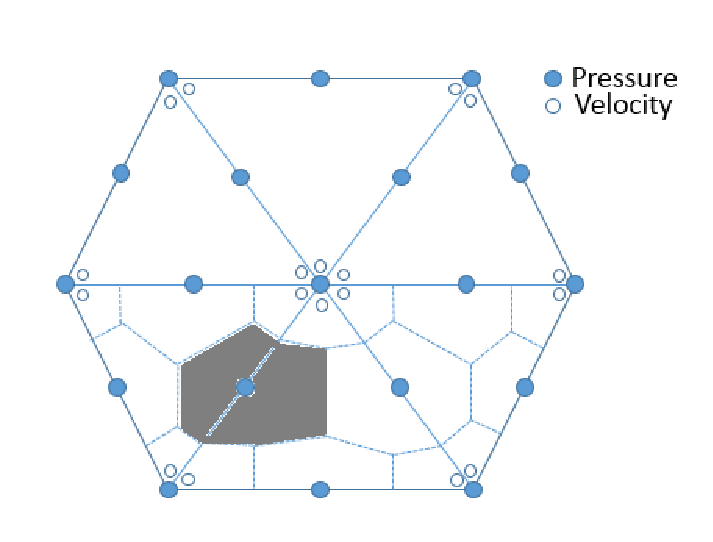
\includegraphics[width=.5\textwidth]{./Pics/P1DGP2.pdf}}
\caption{2D representation of \PN[1]{2} element pairs used in this work. Shaded areas denote control volumes across two contiguous elements. Blue and white circles represent pressure and velocity nodes, respectively.} 
\label{fig:fem_cv}
\end{figure}

\clearpage

%%%%
%%%%  FIGURE
%%%%
\begin{figure}[h]
\centering
\vbox{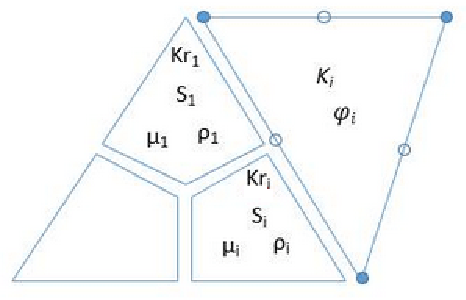
\includegraphics[width=.75\textwidth]{./Pics/element_n.pdf}}
\caption{This is a graphical representation of two different element types. Triangle {\it A} is a representation of the \PN[1]{2} element-pair, whereas triangle {\it B} represents the \PN[1]{1} element-pair. Porosity $\phi_{i}$, permeability {\bf K}$_{i}$, velocity and pressure are primarily represented in FE space whereas scalar fields (such as saturation, density, viscosity etc) are represented in CV space.}
\label{fig:fem_elem}
\end{figure}
\clearpage

%%%%
%%%%  FIGURE 
%%%%
\begin{figure}[h]
\centering
\vbox{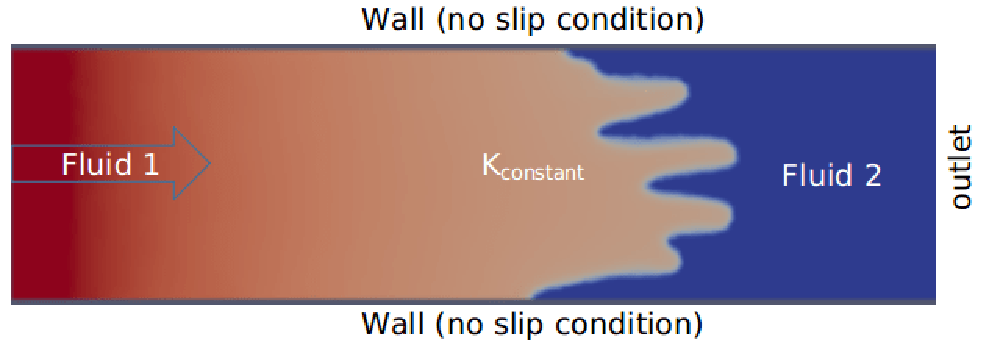
\includegraphics[width=0.75\textwidth]{./Pics/phase_vol_frac_uni_perm_1.pdf}}
\caption{Schematics of formation of flow instabilities during injection of a pure low viscosity fluid (red) into a domain saturated with a second fluid (dark blue). The ratio of viscosity between the two fluids is 5. In this case, the initially piston shape front collapses leading to the formation of several fingers.}
\label{fig:simple_case}
\end{figure}
\clearpage


%%%%
%%%%  FIGURE 
%%%%
\begin{figure}[ht] 
\vbox{
\hbox{\hspace{-0.3cm}
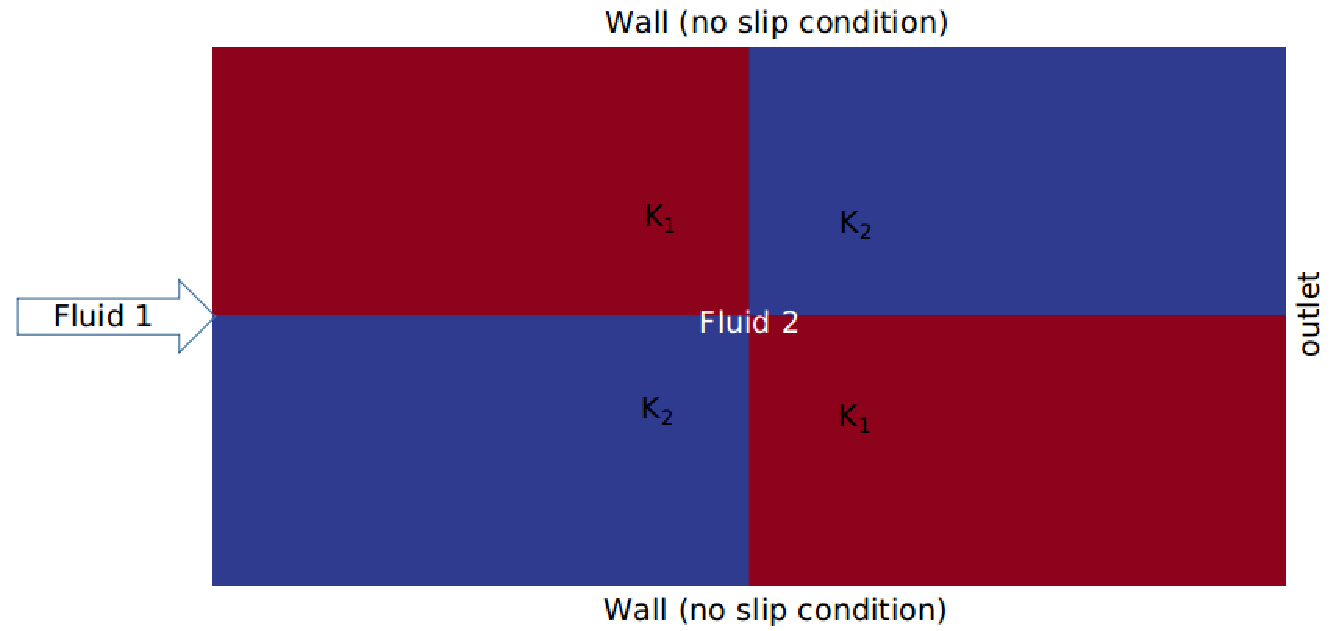
\includegraphics[width=.8\textwidth]{./Pics1/2b2_wi_fine/2b2_whole_in_fine_perm_1.pdf} 
}
\vspace{0.0cm}
\hbox{\hspace{3.5cm} (a) map of permeabilities ($\mathbf{K}$)
}
\vspace{0.25cm}
\hbox{\hspace{1.5cm}
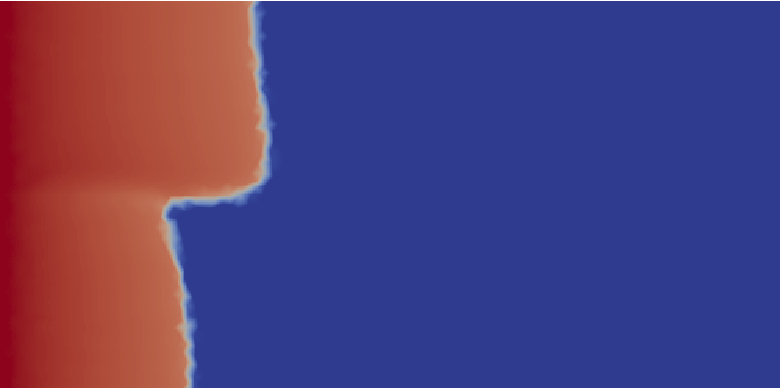
\includegraphics[width=.85\textwidth]{./Pics1/2b2_wi_fine/2b2_whole_in_fine_250_2.pdf}
}
\vspace{0.0cm}
\hbox{\hspace{4.5cm} (b) flow at t=250 
}
\vspace{0.25cm}
\hbox{\hspace{1.5cm}
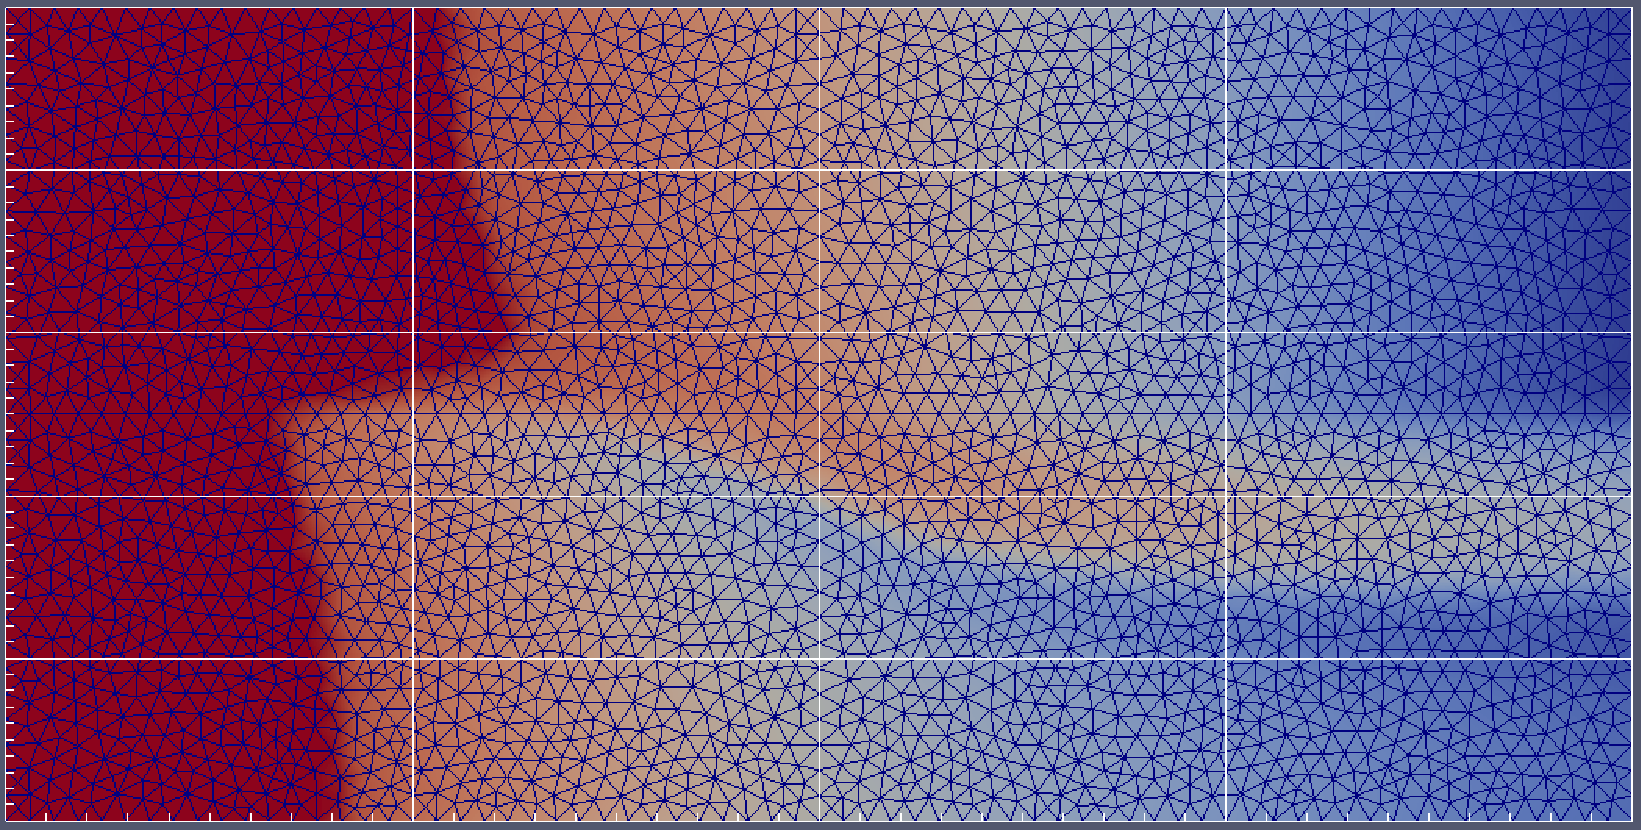
\includegraphics[width=.65\textwidth]{./Pics1/2b2_wi_fine/2b2_whole_in_fine_3000_2.pdf}
}
\vspace{0.0cm}
\hbox{\hspace{4.0cm} (c) flow at t=3000   
}}     
\caption{Model validation of fluid displacement in heterogeneous porous media ({\it VR}=1): (a) the domain is divided into four subdomains with prescribed synthetic permeability, $\mathbf{K}_{1}=1$ and $\mathbf{K}_{2}=2.5$; (b-c) snapshots of saturation (displacing fluid) field at t=$25$s and t=$300$ sec. The domain is discretised with $5960$ \PN[1]{2} elements. }
\label{fem_cv_represent_a}
\end{figure}
\clearpage



%%%%
%%%%  FIGURE
%%%%
\begin{landscape}
\begin{figure}[ht] 
\vbox{\vspace{-1cm}
\hbox{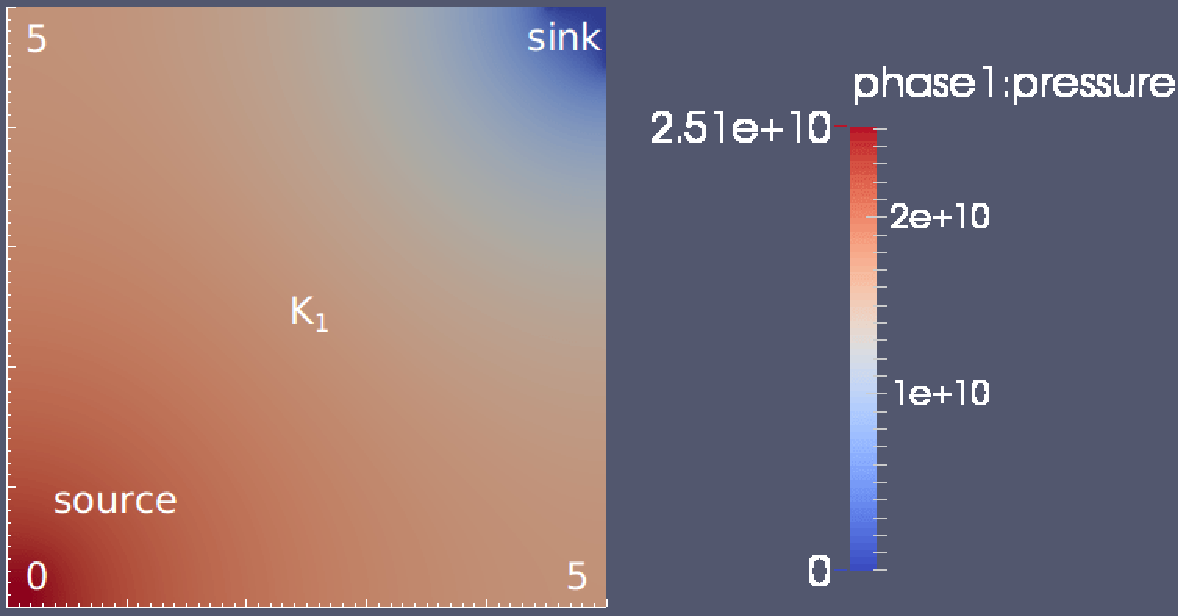
\includegraphics[width=.7\textwidth]{./Pics1/Saffman_homogeneous_MR3/saffman_homo_fixed_2.pdf}
      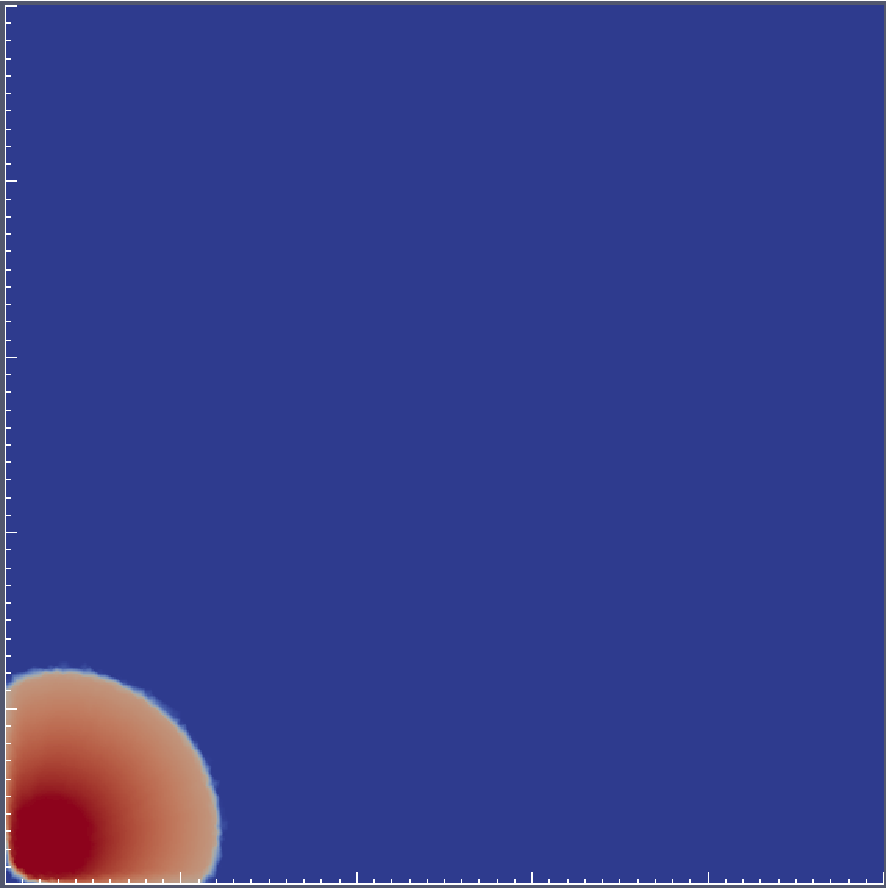
\includegraphics[width=.37\textwidth]{./Pics1/Saffman_homogeneous_MR3/saffman_homo_fixed_250.pdf}
      \includegraphics[width=.37\textwidth]{./Pics1/Saffman_homogeneous_MR3/saffman_homo_fixed_1000.pdf}}
\vspace{0.cm}
\hbox{\hspace{2.5cm} (a) pressure at t=0s \hspace{5.cm} (b) t=0.87s \hspace{2.75cm} (c) t=3.54s}
\vspace{0.5cm}
\hbox{
      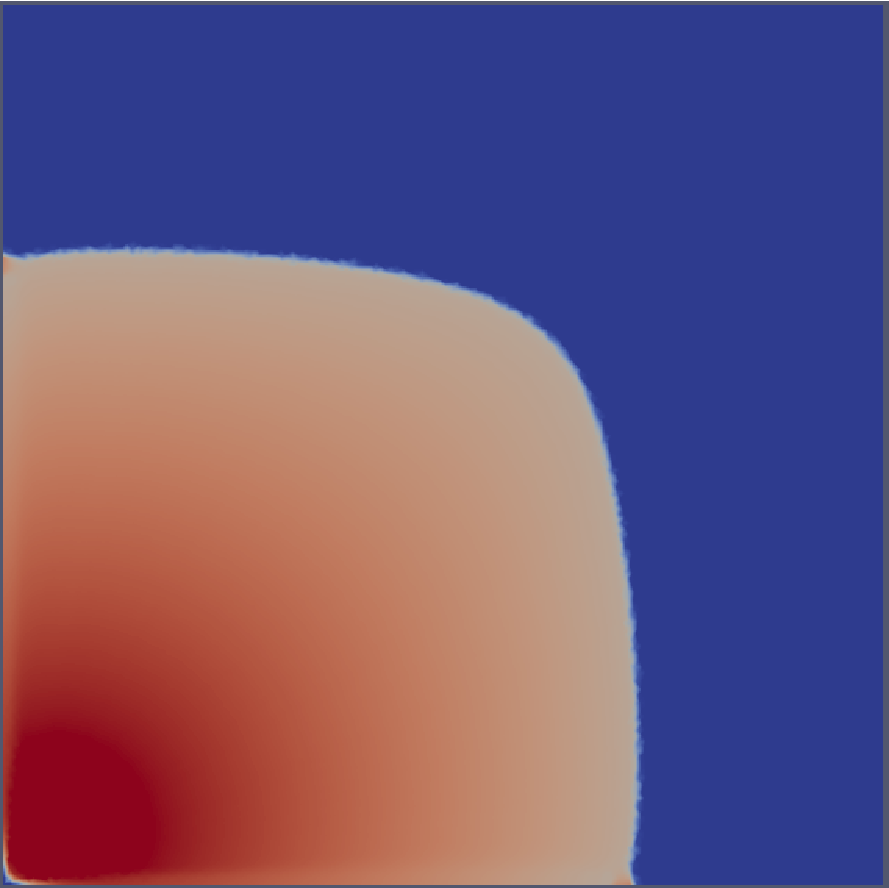
\includegraphics[width=.375\textwidth]{./Pics1/Saffman_homogeneous_MR3/saffman_homo_fixed_2500.pdf}
      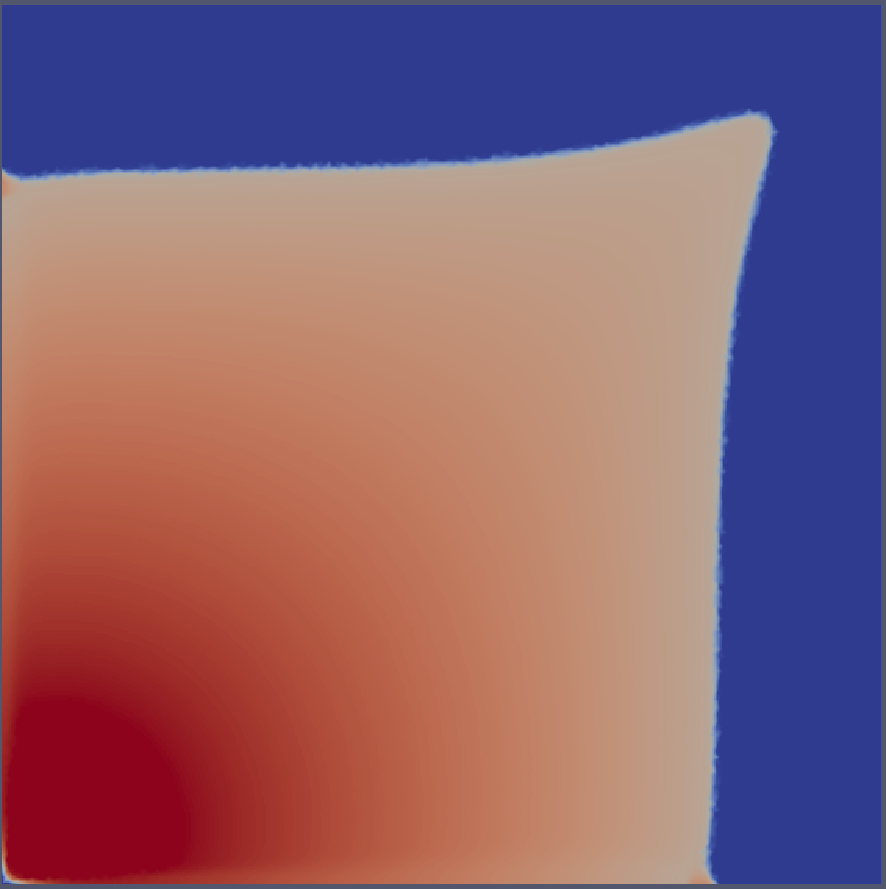
\includegraphics[width=.375\textwidth]{./Pics1/Saffman_homogeneous_MR3/saffman_homo_fixed_3500.pdf} 
      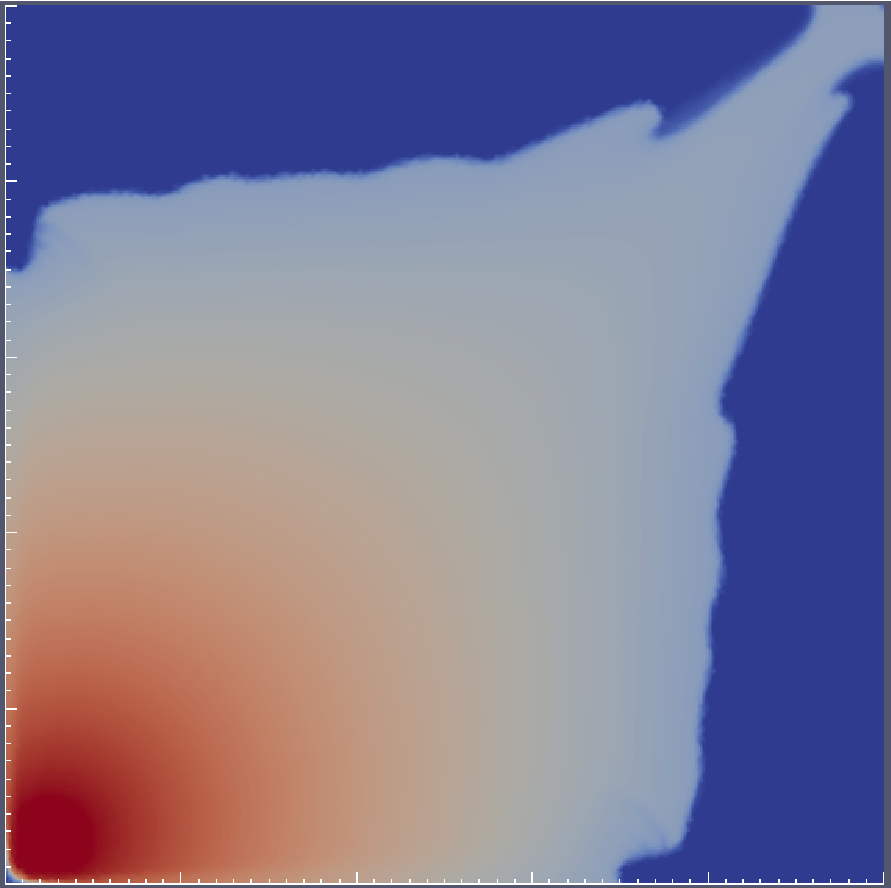
\includegraphics[width=.65\textwidth]{./Pics1/Saffman_homogeneous_MR3/saffman_homo_fixed_end.pdf}}
\vspace{0.cm}
\hbox{ \hspace{1.cm} (d) t=8.86s \hspace{3.0cm} (e) t=12.41s   \hspace{4.0cm} (f) t=17.95s}
\vspace{0.cm}
}   
\caption{Simulated flow in a Hele-Shaw cell ({\it VR}=3): (a) initial pressure profile $\left(\text{in g.cm}^{-1}\text{.s}^{-2}\right)$ with source and sink regions are explicitly shown along with dimensions (in cm); (b-f) snapshots of wetting phase saturation showing flow profile as the simulation evolves. The domain contains $47500$ \PN[1]{2} triangular elements.}
\label{fig:homoheleshaw_VN3}
\end{figure}
\end{landscape}
\clearpage



%%%%
%%%%  FIGURE
%%%%
\begin{landscape}
\begin{figure}[ht] 
\vbox{\vspace{-1cm}
\hbox{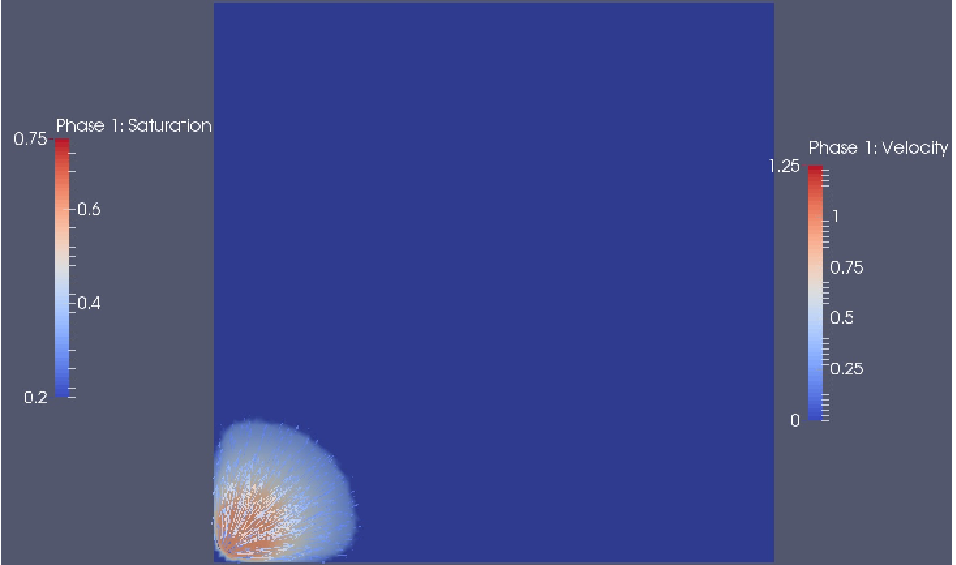
\includegraphics[width=.9\textwidth, height=0.5\textwidth]{./Pics1/Saffman_homogeneous_VR10/ST_Homog_VR10_D201c.pdf}
\hspace{0.5cm}      
      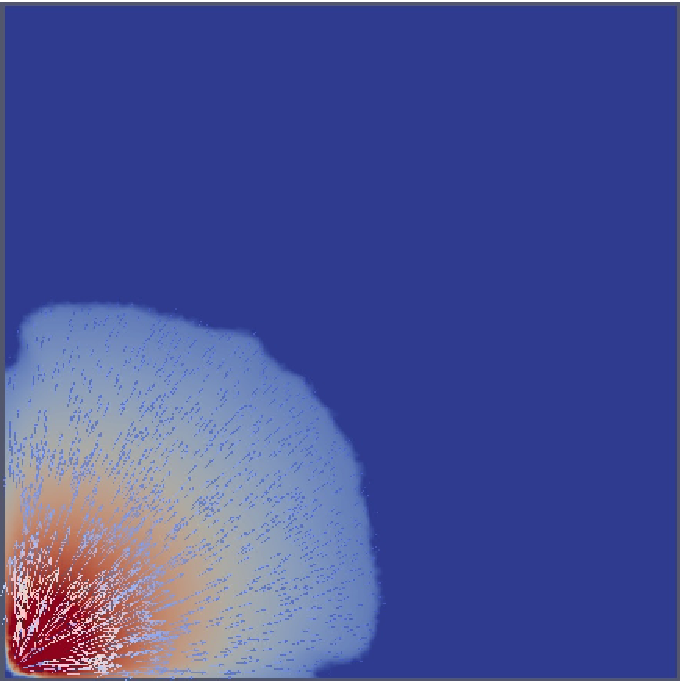
\includegraphics[width=.5\textwidth]{./Pics1/Saffman_homogeneous_VR10/ST_Homog_VR10_D1001c.pdf}}
\vspace{0.cm}
\hbox{\hspace{5.cm} (a) t=0.66s \hspace{8.cm} (b) t=3.43s }
\vspace{0.5cm}
\hbox{
      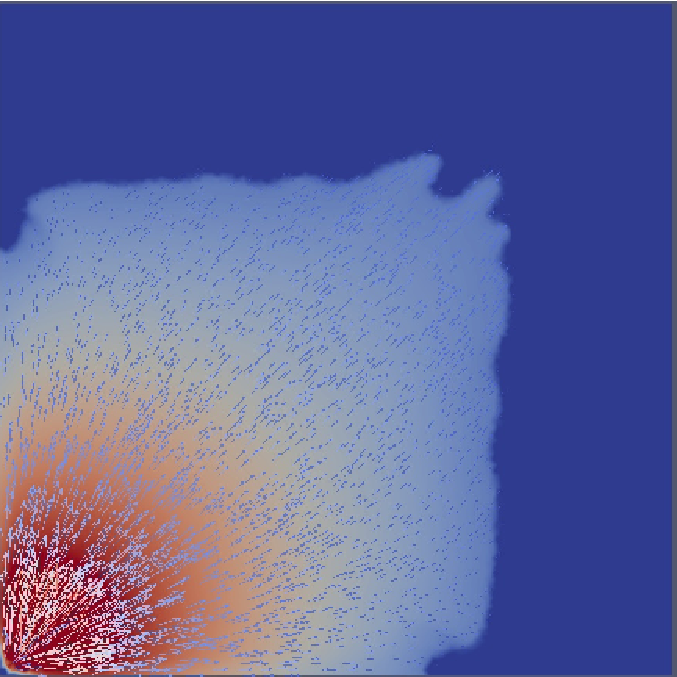
\includegraphics[width=.5\textwidth]{./Pics1/Saffman_homogeneous_VR10/ST_Homog_VR10_D2001c}
      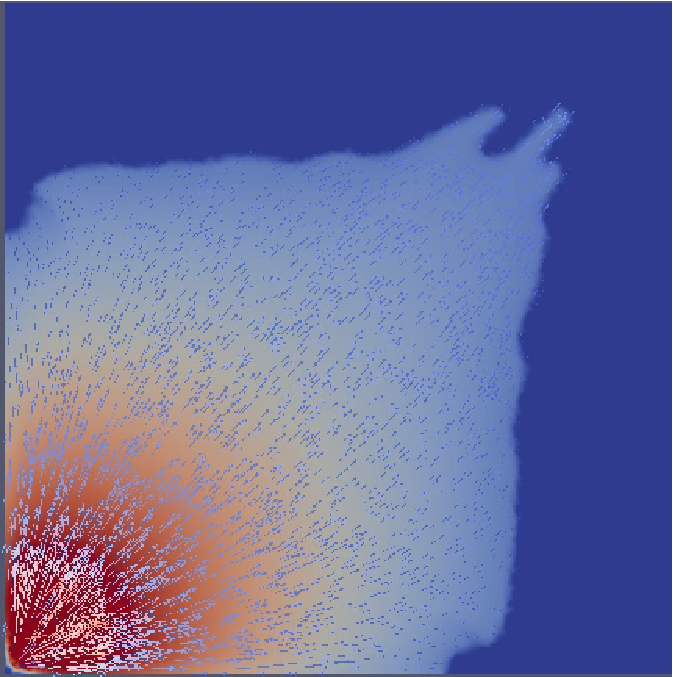
\includegraphics[width=.5\textwidth]{./Pics1/Saffman_homogeneous_VR10/ST_Homog_VR10_D2201c}
      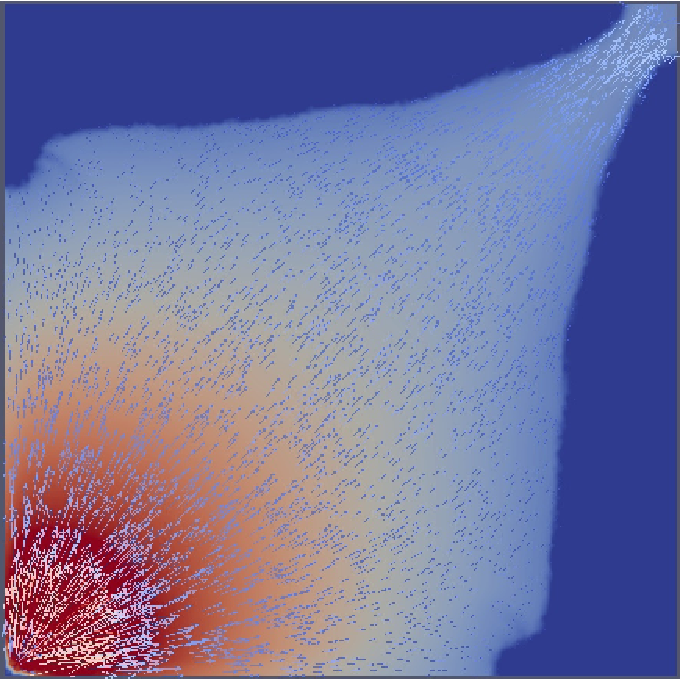
\includegraphics[width=.5\textwidth]{./Pics1/Saffman_homogeneous_VR10/ST_Homog_VR10_D3001c}}
\vspace{0.cm}
\hbox{ \hspace{2.cm} (c) t=6.92s \hspace{4.5cm} (d) t=7.61s \hspace{4.5cm} (e)t=10.00s}
\vspace{0.cm}
}   
\caption{Simulated flow in a Hele-Shaw cell ({\it VR}=10): snapshots of overlapped wetting phase saturation and velocity vectors showing flow profile as the simulation evolves. The domain contains $26313$ \PN[1]{2} triangular elements.}
\label{fig:homoheleshaw_VN10}
\end{figure}
\end{landscape}
\clearpage

%%%%
%%%%  FIGURE
%%%%
\begin{landscape}
\begin{figure}[ht] 
\vbox{\vspace{-1cm}
\hbox{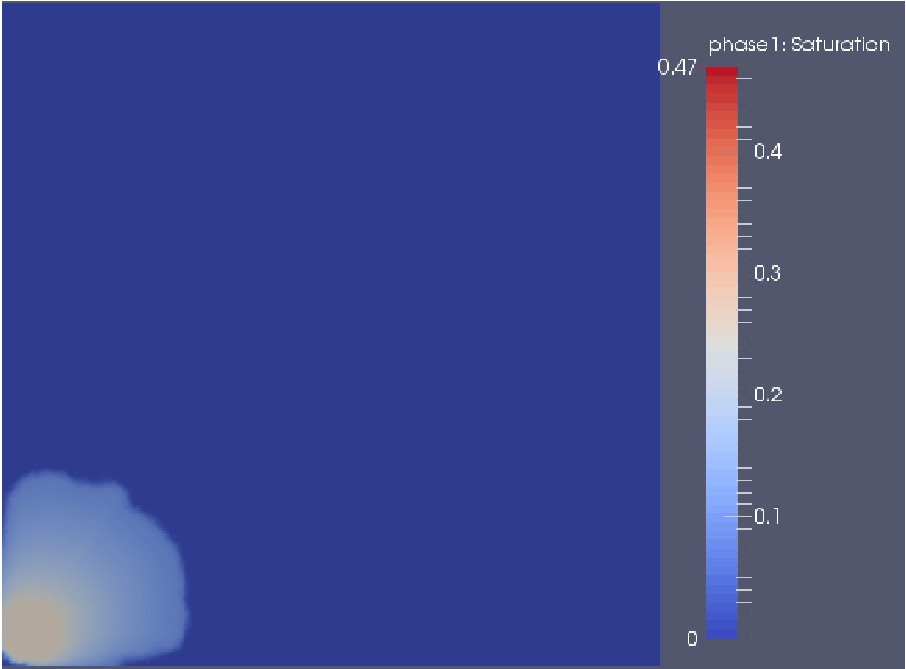
\includegraphics[width=.9\textwidth, height=0.5\textwidth]{./Pics1/Saffman_homogeneous_VR150/ST_Homog_VR150_D300b}
\hspace{0.5cm}      
      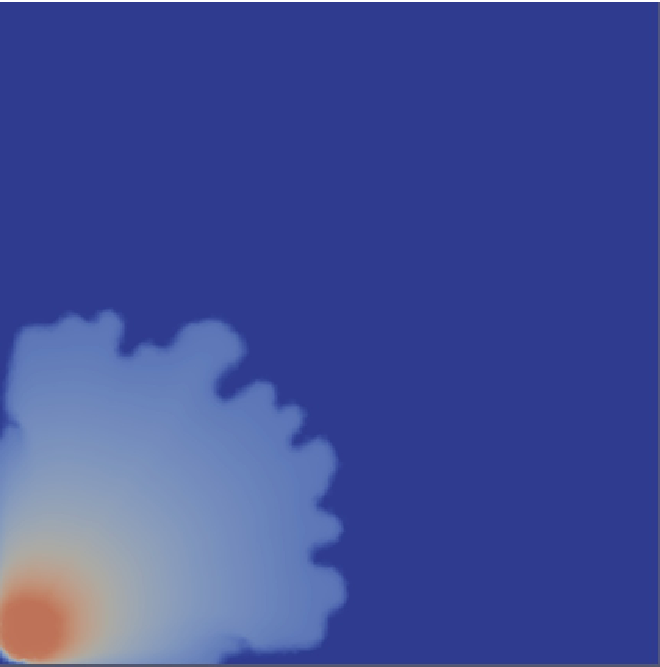
\includegraphics[width=.5\textwidth]{./Pics1/Saffman_homogeneous_VR150/ST_Homog_VR150_D1600b}}
\vspace{0.cm}
\hbox{\hspace{5.cm} (a) t=0.27s \hspace{8.cm} (b) t=0.94s }
\vspace{0.5cm}
\hbox{
      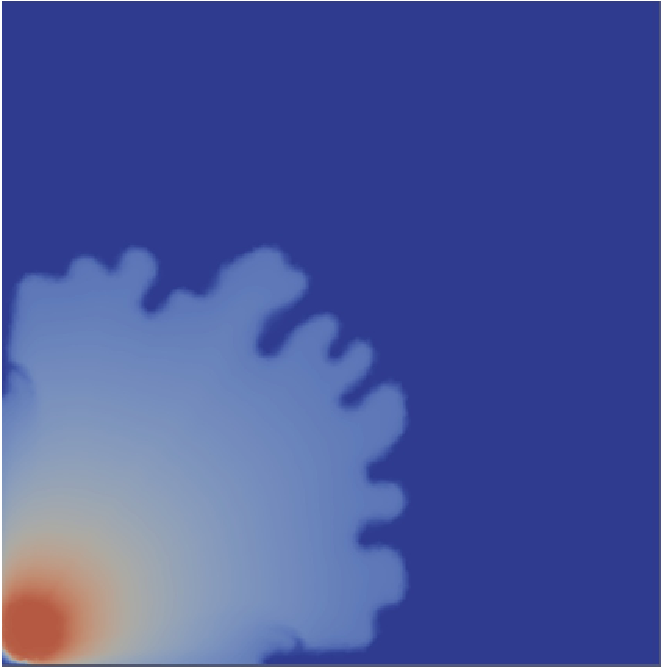
\includegraphics[width=.5\textwidth]{./Pics1/Saffman_homogeneous_VR150/ST_Homog_VR150_D2700b}
      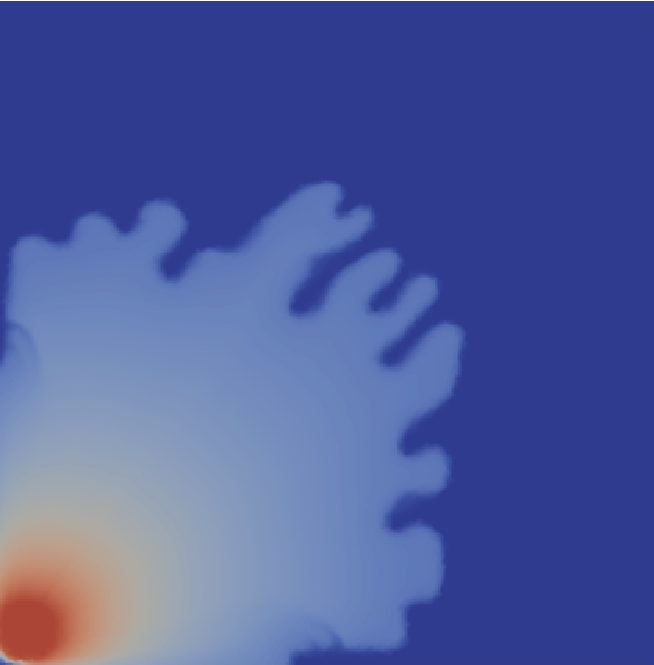
\includegraphics[width=.5\textwidth]{./Pics1/Saffman_homogeneous_VR150/ST_Homog_VR150_D4000b}
      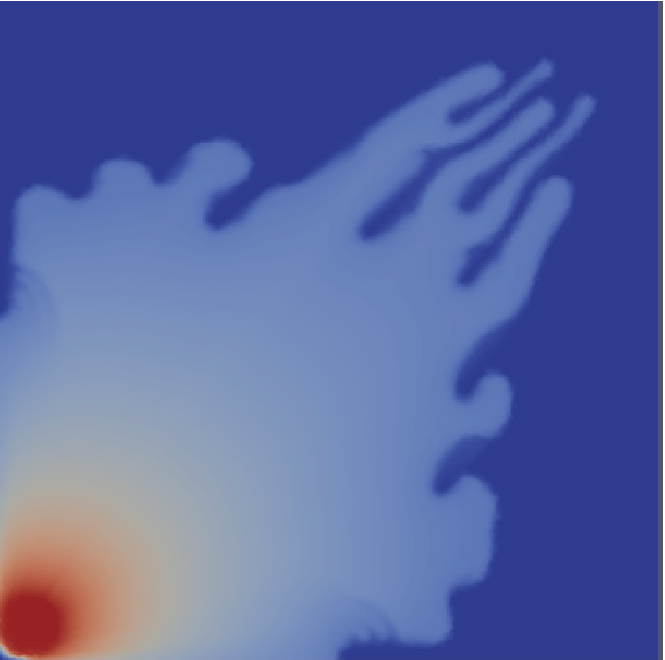
\includegraphics[width=.5\textwidth]{./Pics1/Saffman_homogeneous_VR150/ST_Homog_VR150_D7000b}}
\vspace{0.cm}
\hbox{ \hspace{2.cm} (c) t=1.32s \hspace{4.5cm} (d) t=1.70s \hspace{4.5cm} (e)t=2.31s}
\vspace{0.cm}
}   
\caption{Simulated flow in a Hele-Shaw cell ({\it VR}=150): snapshots of wetting phase saturation showing flow profile as the simulation evolves. The domain contains $26313$ \PN[1]{2} triangular elements.}
\label{fig:homoheleshaw_VN10}
\end{figure}
\end{landscape}
\clearpage


%%%%
%%%%  FIGURE
%%%%
\begin{landscape}
\begin{figure}[ht] 
\hbox{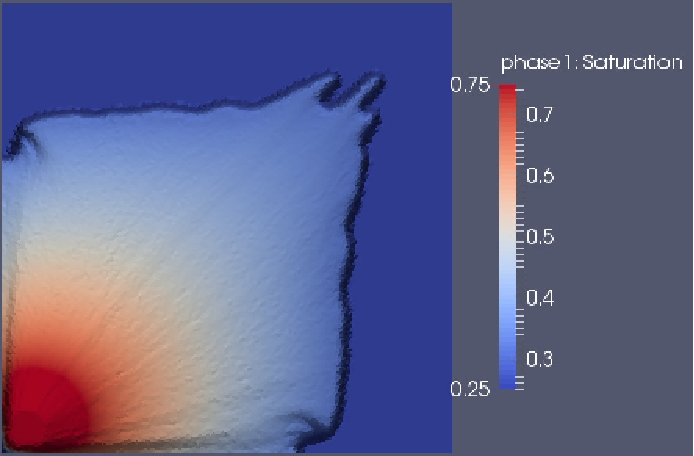
\includegraphics[width=.5\textwidth]{./Pics1/Saffman_homogeneous_VR10/ST_Homog_VR10_D2201_bbd}
       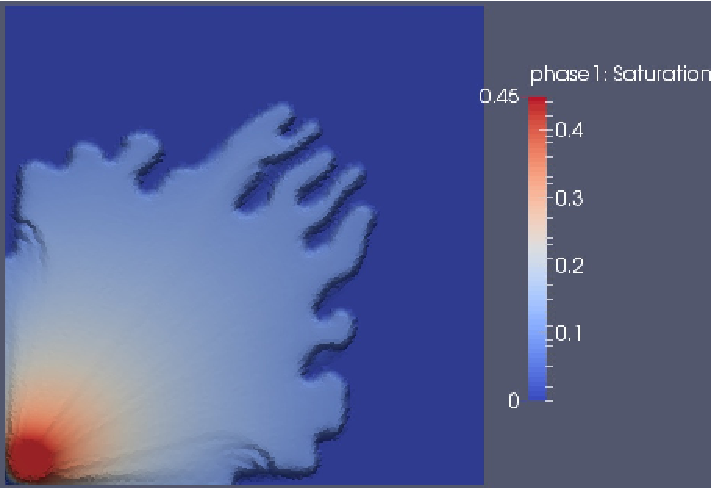
\includegraphics[width=.49\textwidth]{./Pics1/Saffman_homogeneous_VR150/ST_Homog_VR150_D5003_k2b}}
\caption{Simulated flow in Hele-Shaw cells performed with viscosity ratios of 10 (left, t=7.61s) and 150 (t=1.94s). Width of largest fingers are approximetely 0.70 and 0.90cm, which are in good agreement with values obtained from \citet{guan_2003}'s analytic solution. Domains of both simulations contain $26313$ \PN[1]{2} triangular elements.\red{(More pics to be added!!)}}
\label{fig:homoheleshaw_VN10_VN150}
\end{figure}
\end{landscape}



\begin{comment}

%%%%
%%%%  FIGURE
%%%%
\begin{landscape}
\begin{figure}[ht] 
\vbox{\vspace{-1cm}
\hbox{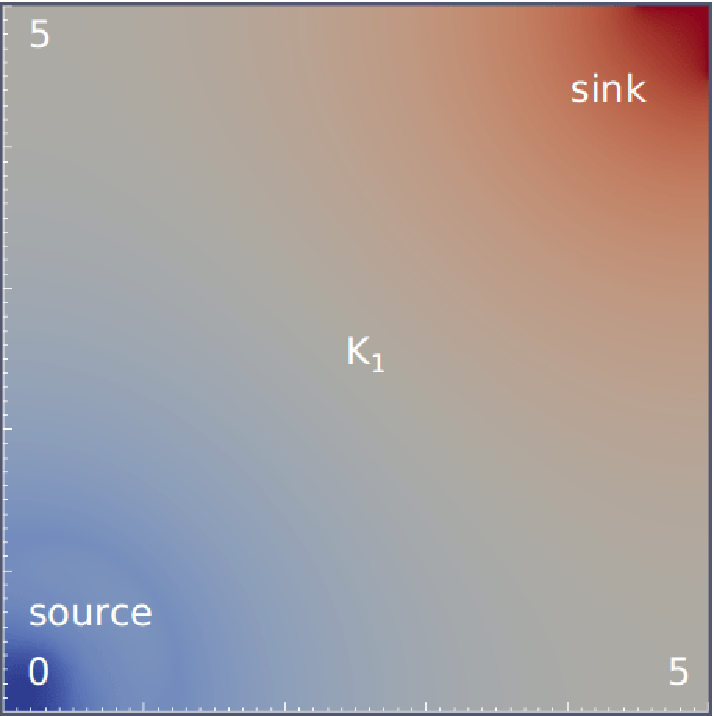
\includegraphics[width=.5\textwidth]{./Pics1/Saffman_homogeneous/saffman_homo_fixed_1.pdf}
      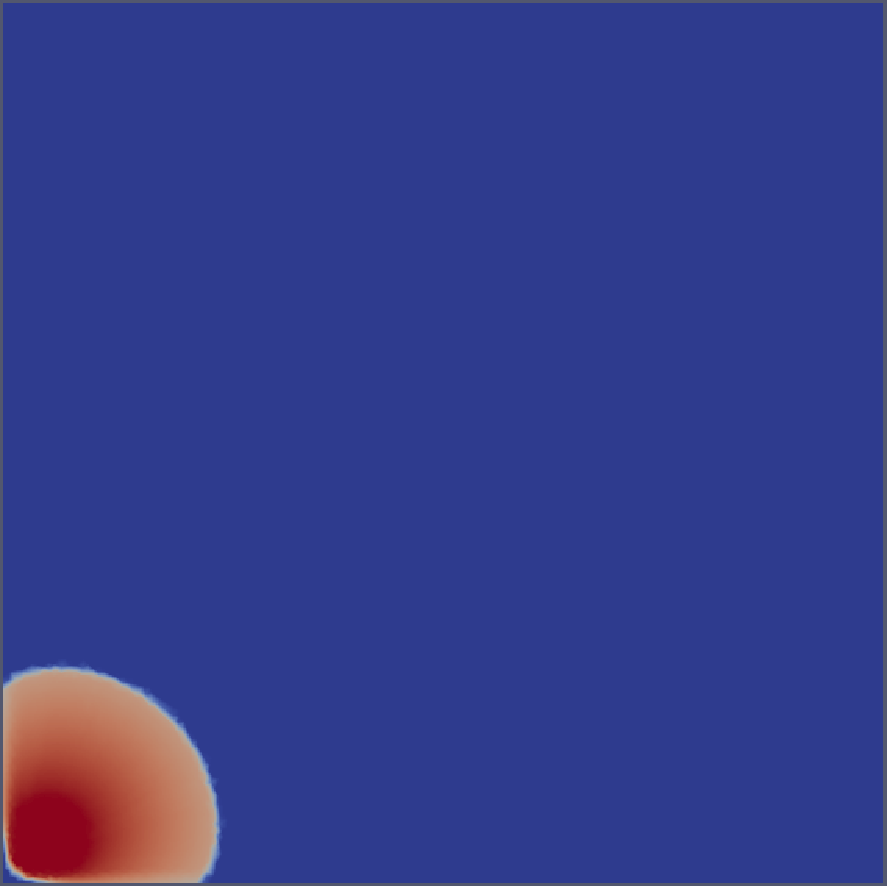
\includegraphics[width=.5\textwidth]{./Pics1/Saffman_homogeneous/saffman_homo_fixed_250_1.pdf}
      \includegraphics[width=.5\textwidth]{./Pics1/Saffman_homogeneous/saffman_homo_fixed_1000.pdf}}
\vspace{0.cm}
\hbox{\hspace{1.0cm} (a) pressure at t=0 \hspace{3.cm} (b) t=250\red{(???)} \hspace{3.0cm} (c) t=1000\red{(???)}}
\vspace{0.5cm}
\hbox{
      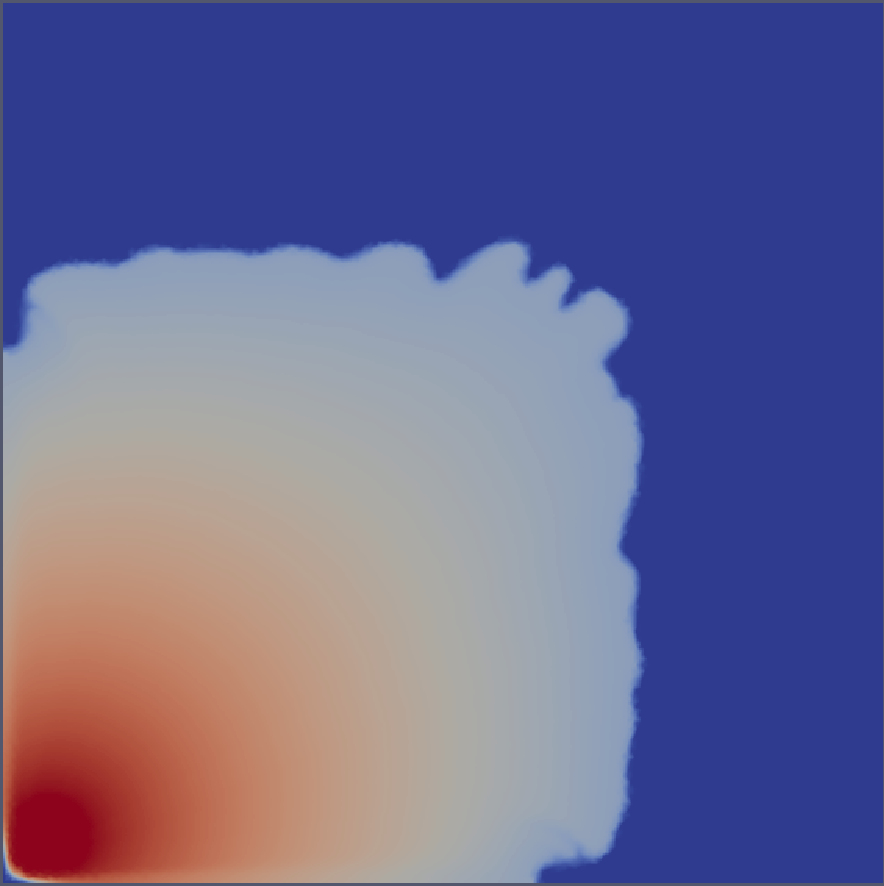
\includegraphics[width=.5\textwidth]{./Pics1/Saffman_homogeneous/saffman_homo_fixed_6000.pdf}
      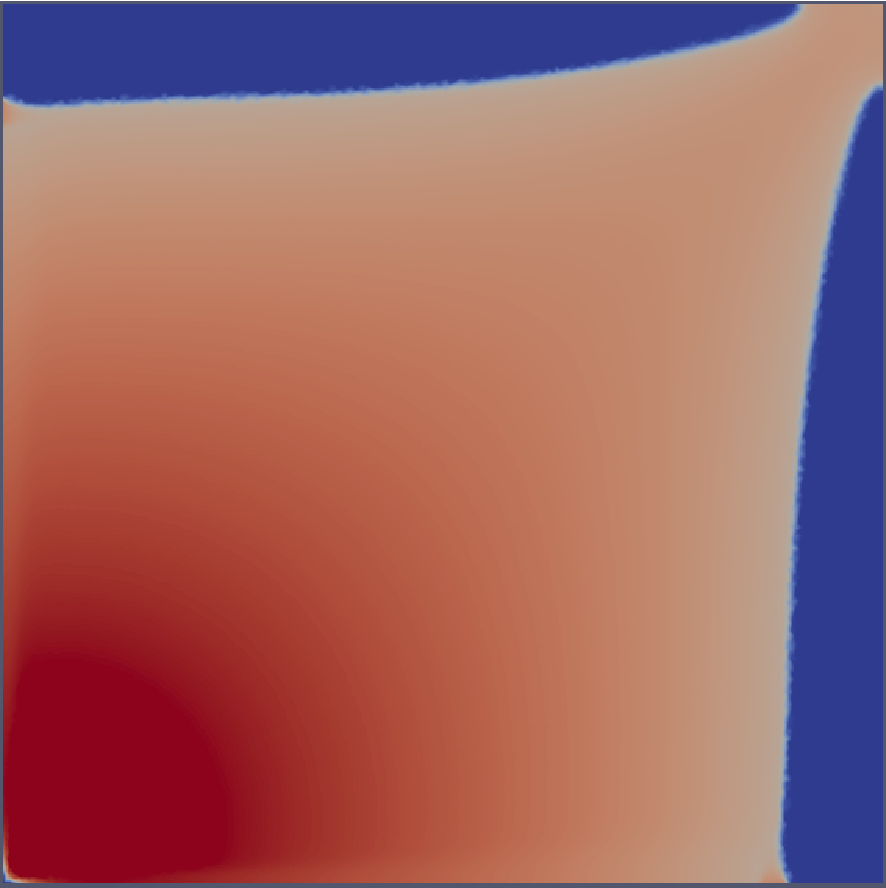
\includegraphics[width=.5\textwidth]{./Pics1/Saffman_homogeneous/saffman_homo_fixed_end_1.pdf}}
\vspace{0.cm}
\hbox{ \hspace{2.cm} (d) t=6000\red{(???)} \hspace{3.cm} (e) t=XXX\red{(???)}}
\vspace{0.cm}
}   
\caption{Simulated flow in a Hele-Shaw cell ({\it VR}=10): (a) pressure profile $\left(\text{in g.cm}^{-1}\text{.s}^{-2}\right)$ with source and sink regions explicitly shown along with dimensions (in cm); (b-e) snapshots of wetting phase saturation showing flow profile as the simulation evolves. The domain contains $47000$ \PN[1]{2} triangular elements. The pressure and saturation range of values are the same like the  case in fig.\ref{fig:homoheleshaw_VN3}.}
\label{fig:homoheleshaw_VN10}
\end{figure}
\end{landscape}
\clearpage
\end{comment}


%%%
%%% FIGURE XXXXXX
%%%
\begin{landscape}
  \begin{figure}[ht]
  \vbox{\vspace{-1cm}
      \hbox{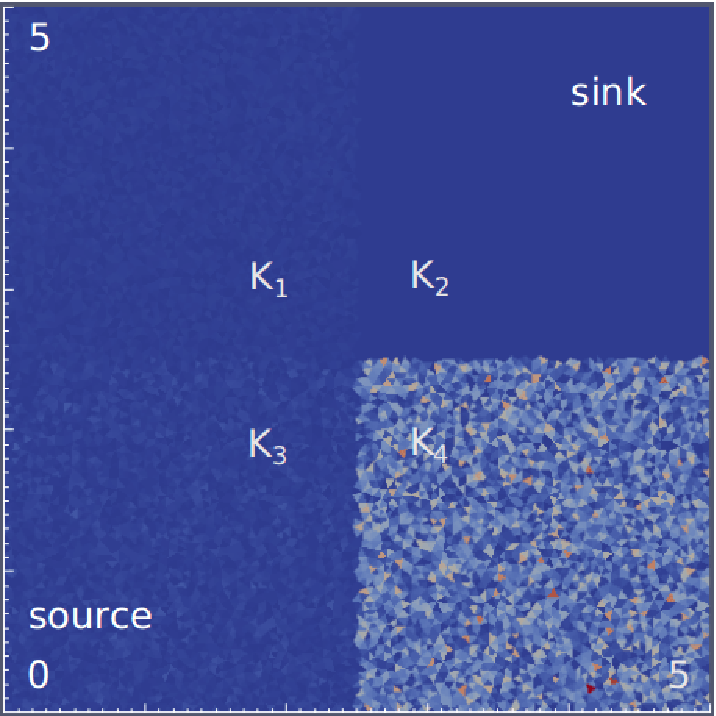
\includegraphics[width=.5\textwidth]{./Pics1/Saffman_heterogeneous/saffman_heter_fixed_1.pdf}
            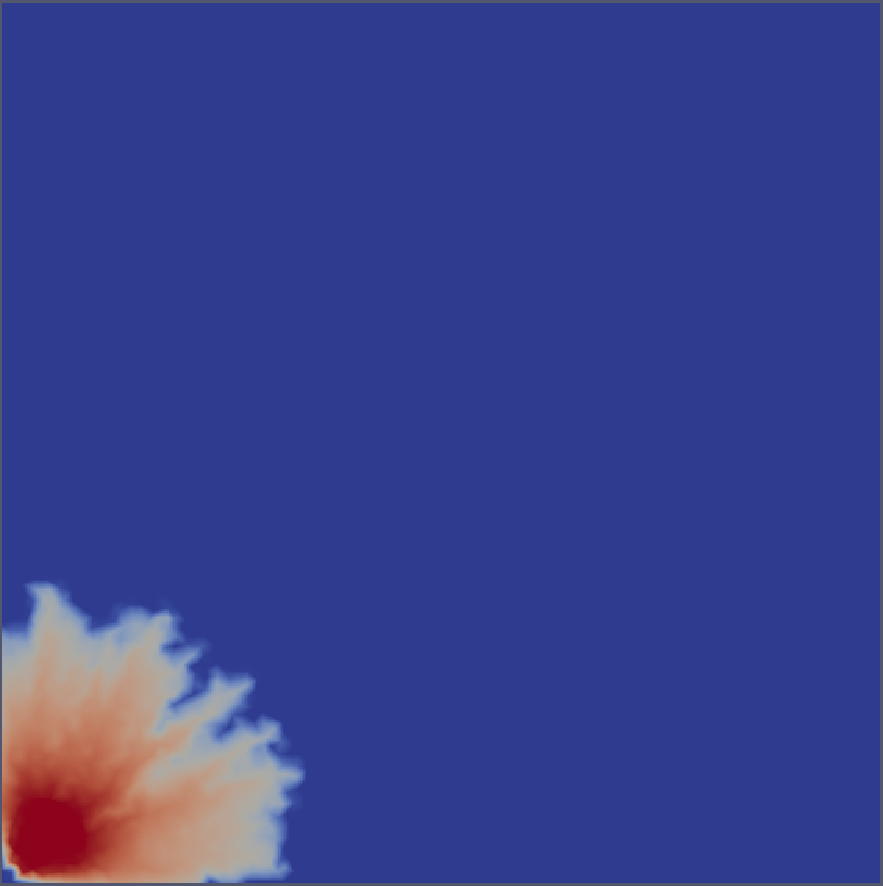
\includegraphics[width=.5\textwidth]{./Pics1/Saffman_heterogeneous/saffman_heter_fixed_500.pdf} 
            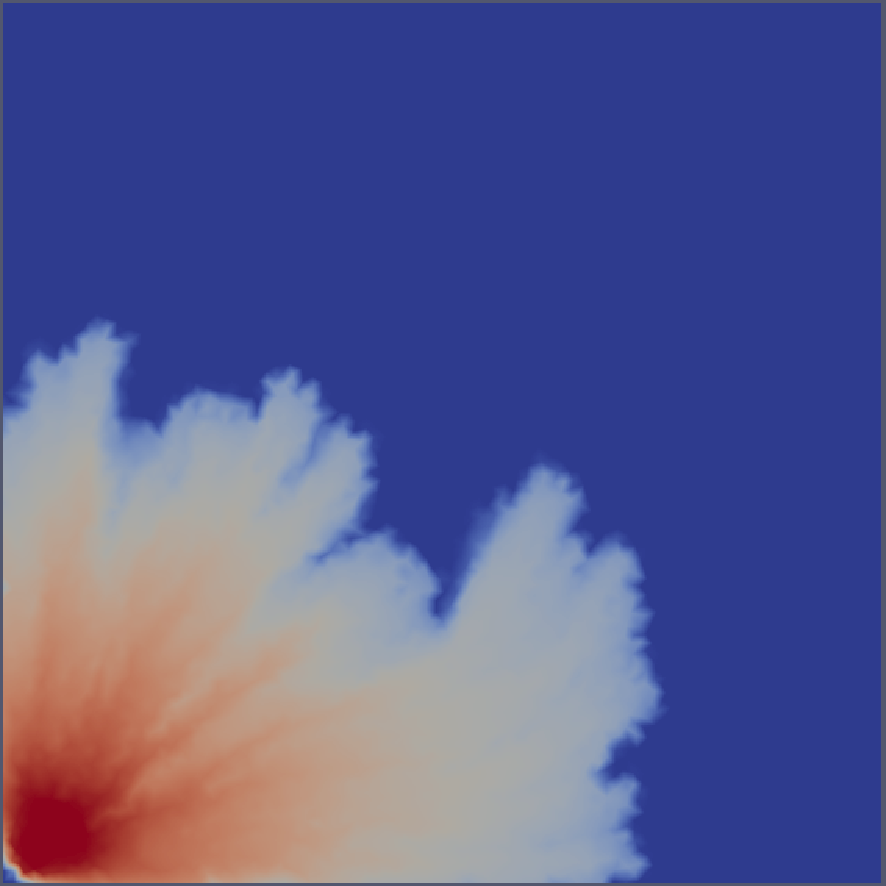
\includegraphics[width=.5\textwidth]{./Pics1/Saffman_heterogeneous/saffman_heter_fixed_2000.pdf} }
      \hbox{\hspace{1.0cm} (a) permeability map \hspace{3.cm} (b) t=0.75s \hspace{4.0cm} (c) t=8s}
      \vspace{0.5cm}
      \hbox{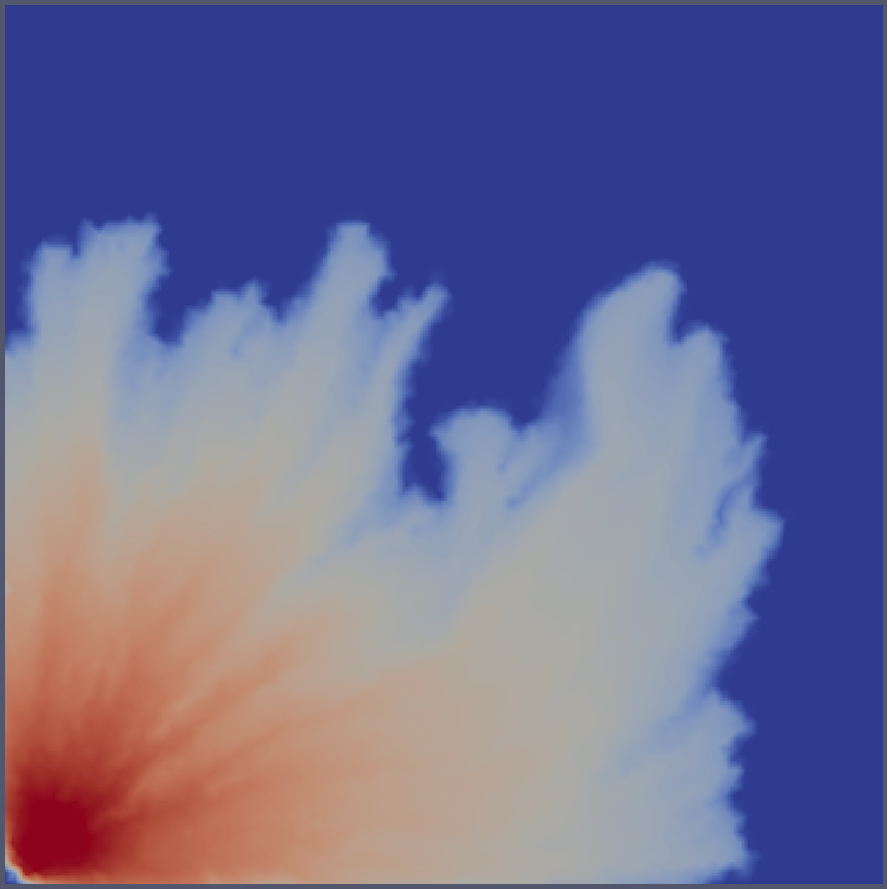
\includegraphics[width=.5\textwidth]{./Pics1/Saffman_heterogeneous/saffman_heter_fixed_3000.pdf}
            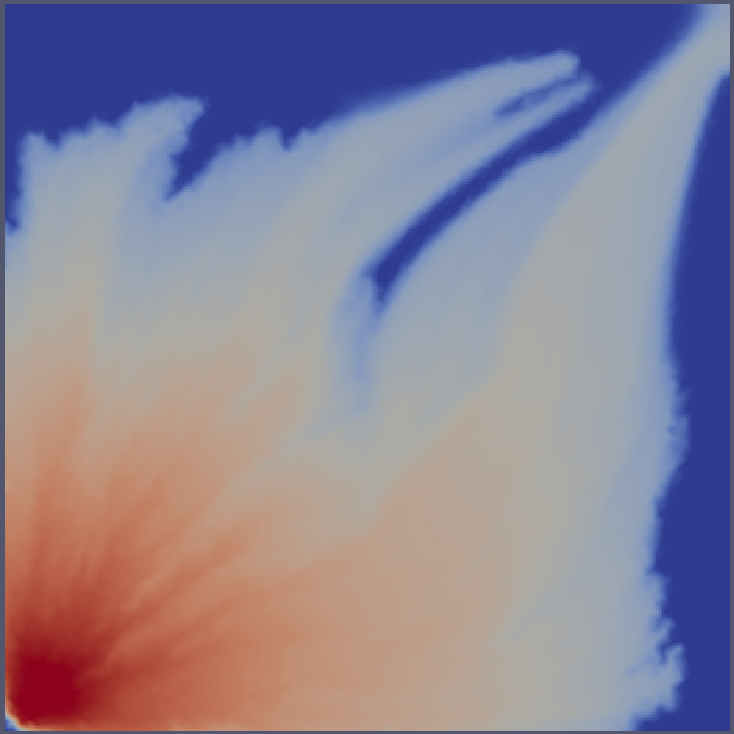
\includegraphics[width=.5\textwidth]{./Pics1/Saffman_heterogeneous/saffman_heter_fixed_6000.pdf}
            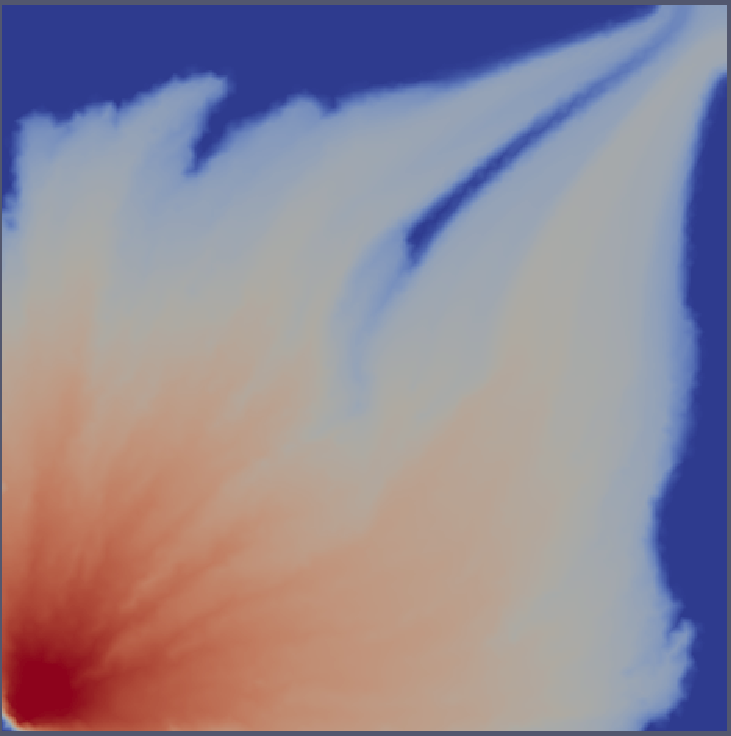
\includegraphics[width=.5\textwidth]{./Pics1/Saffman_heterogeneous/saffman_heter_fixed_24000.pdf} }
      \hbox{\hspace{2.5cm} (d) t=18s \hspace{5.cm} (e) t= \hspace{3.0cm} (f) t=24000 }}
\caption{Simulated flow in a modified Hele-Shaw cell with {\it VR}=10: (a) permeability distribution $\left(\text{10}^{-10}\le\mathbf{K}_{1}\le\text{5}\times\text{10}^{-10}\right.$, {\bf K}$_{2}$=10$^{-10}$, 10$^{-11}\le\mathbf{K}_{3}\le$ 5$\times$10$^{-10}$ and 10$^{-12}\le\mathbf{K}_{4}\le$ 5$\times$10$\left.^{-10}\text{ cm}^{2}\right)$; (b-f) snapshots of saturation profile during \red{XX} seconds of simulation. The domain contains \red{XX} \PN[1]{2} element-pairs.}
\label{fig:HeleShawHeter_VR10}
\end{figure}
\end{landscape}
\clearpage



%%%%
%%%%  FIGURE
%%%%
\begin{landscape}
\begin{figure}[ht] 
\vbox{
\hbox{\hspace{4.0cm}
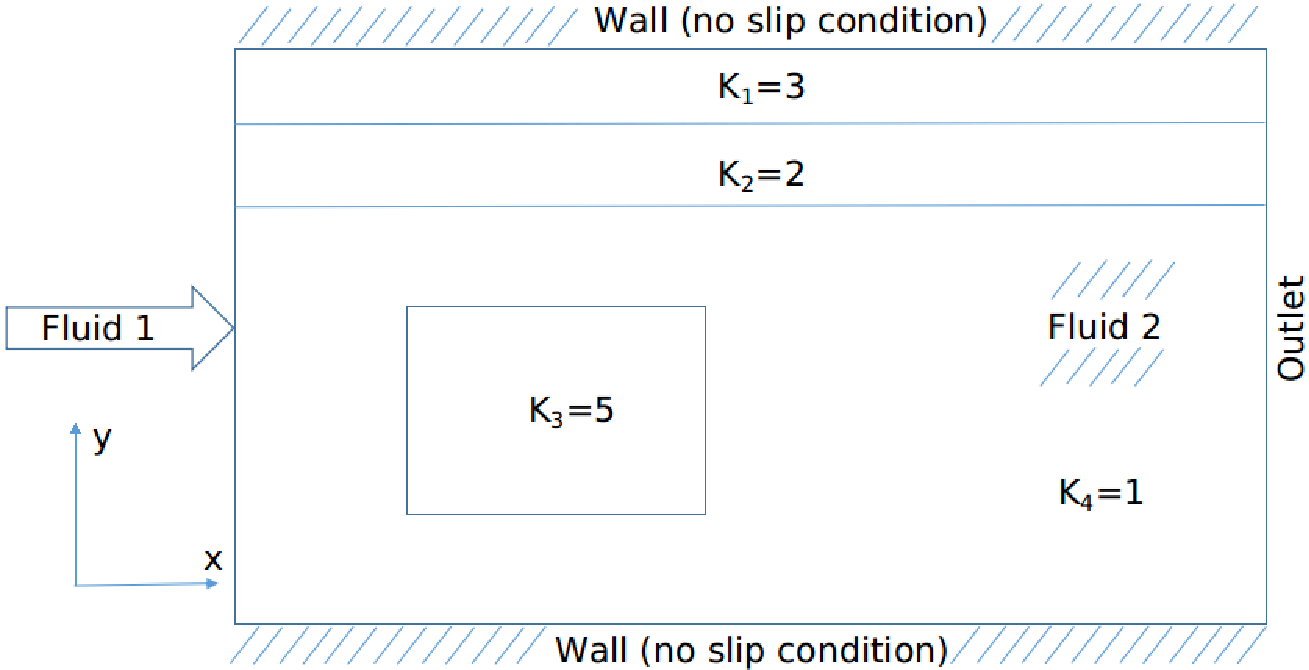
\includegraphics[width=.75\textwidth]{./Pics/map_of_boundaries.pdf} 
}
\vspace{0.0cm}
\hbox{\hspace{6.5cm} (a) map of permeabilties K   
}
\vspace{0.25cm}
\hbox{\hspace{4.0cm}
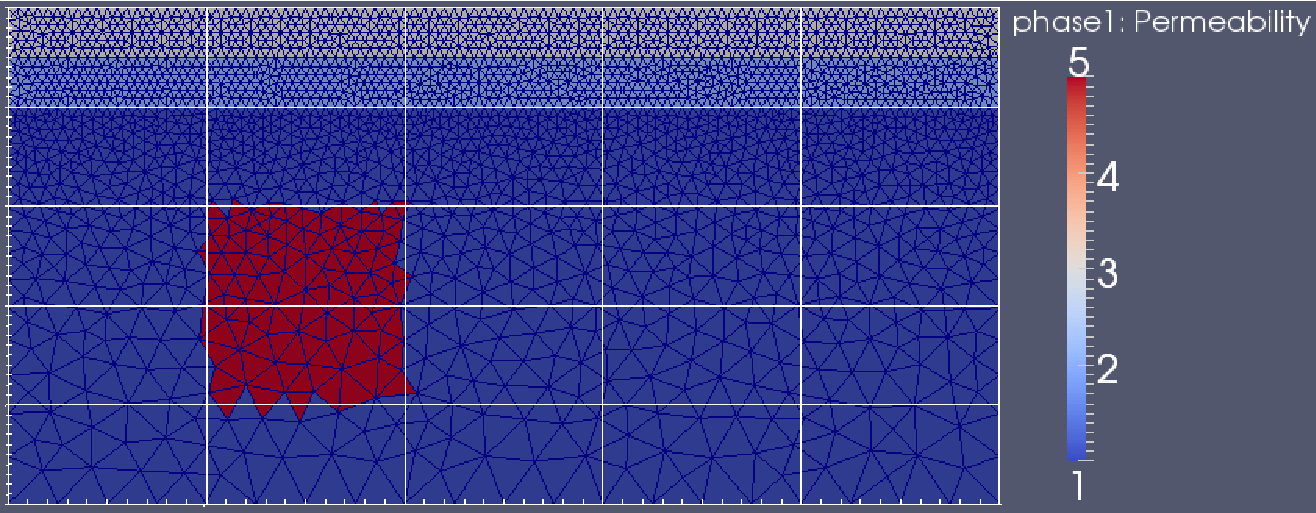
\includegraphics[width=.9\textwidth]{./Pics/map_of_boundaries_1.pdf}
}
\vspace{0.0cm}
\hbox{\hspace{9cm} (b)      
}
}     
\caption{Figure (a) describes the initial and boundary conditions as these are applied in this set of simulations. Below (b) there is a comparison between the unstructured and fixed mesh and the unstructured and adaptive mesh. During the implementation of fixed mesh initially there $4606$ elements while for the adaptive mesh there are $606$ while the majority of them is on the interface between between the two fluids. }
\label{fig:testcase_heter_domain}
\end{figure}
\end{landscape}
\clearpage



%%%%
%%%%  FIGURE
%%%%
\begin{landscape}
\begin{figure}[ht] 
\vbox{
\hbox{\hspace{3.5cm}
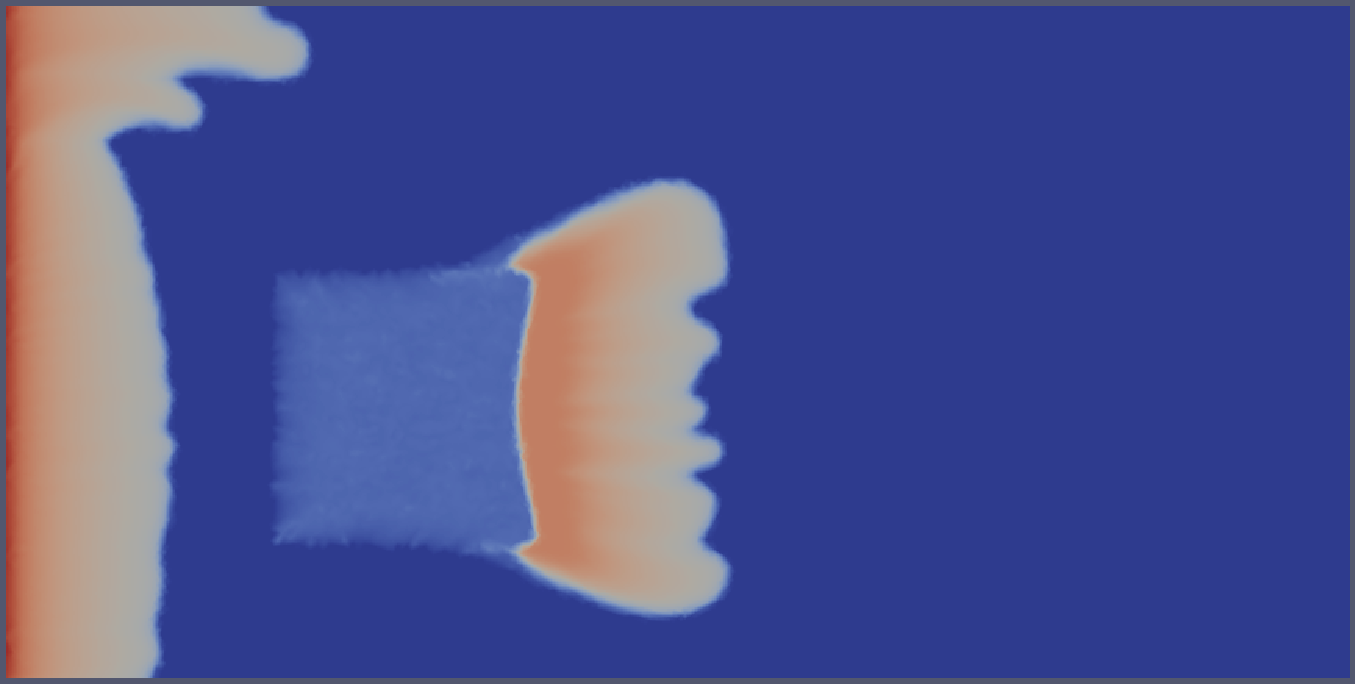
\includegraphics[width=.65\textwidth]{./Pics1/mr10_5regions_fixed/5regions_fixed_250.pdf} 
}
\vspace{0.0cm}
\hbox{\hspace{6.5cm} (a) flow at t=250 (fixed mesh)  
}
\vspace{0.25cm}
\hbox{\hspace{3.5cm}
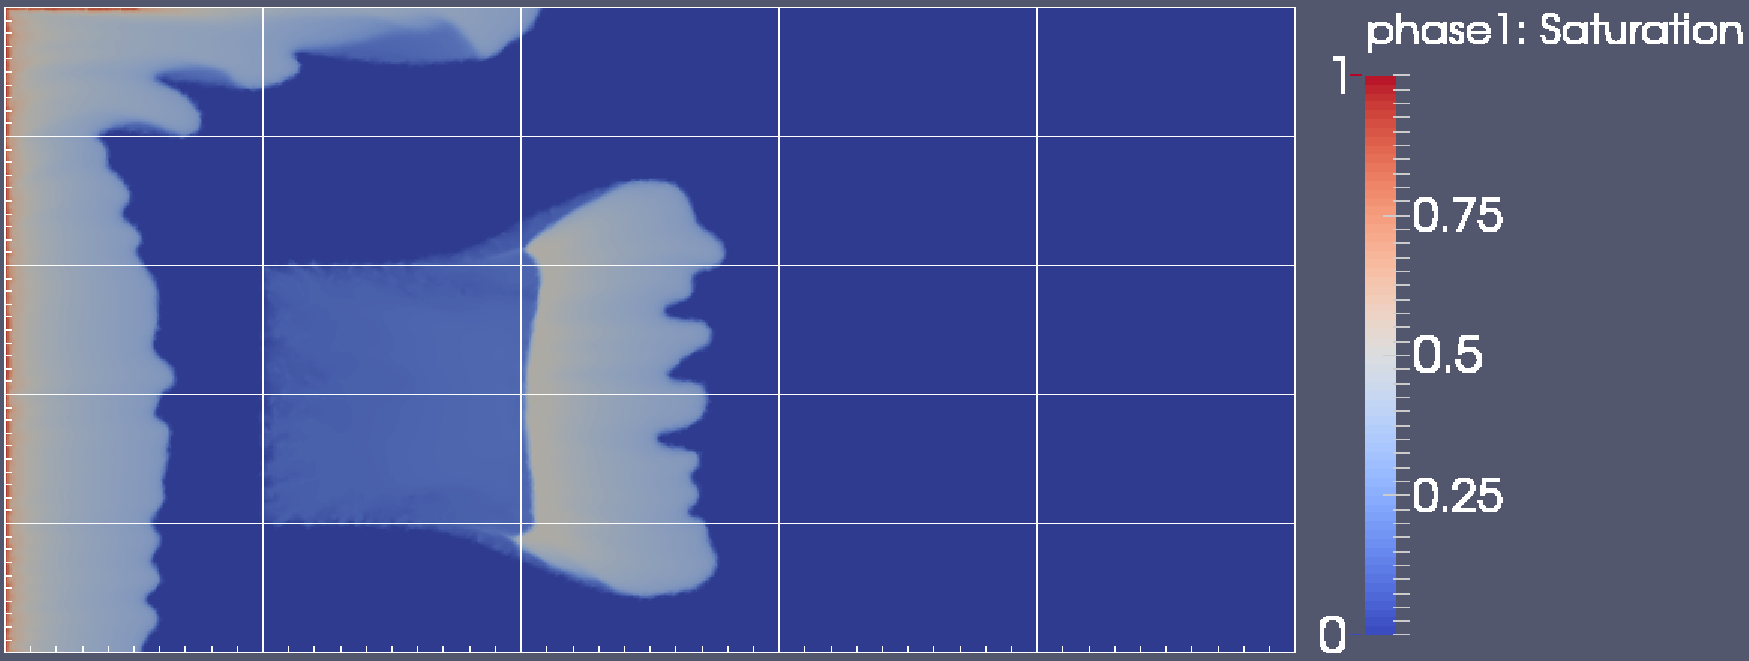
\includegraphics[width=.9\textwidth]{./Pics1/mr10_5regions_adapt/5regions_adapt_250_1.pdf}
}
\vspace{0.0cm}
\hbox{\hspace{6.5cm} (b) flow at t=250 (adaptive mesh)    
}
}     
\caption{For $t=0.125$s, $2$ test-cases under the VR=$10$ and under fixed (top) and adaptive(bottom) mesh are compared. There is a significant difference on the main front (left hand side of the domain) and the number of finger that appear.}
\label{fig:2testcase_a}
\end{figure}
\end{landscape}
\clearpage


%%%%
%%%%  FIGURE
%%%%
\begin{landscape}
\begin{figure}[ht] 
\vbox{
\hbox{\hspace{3.5cm}
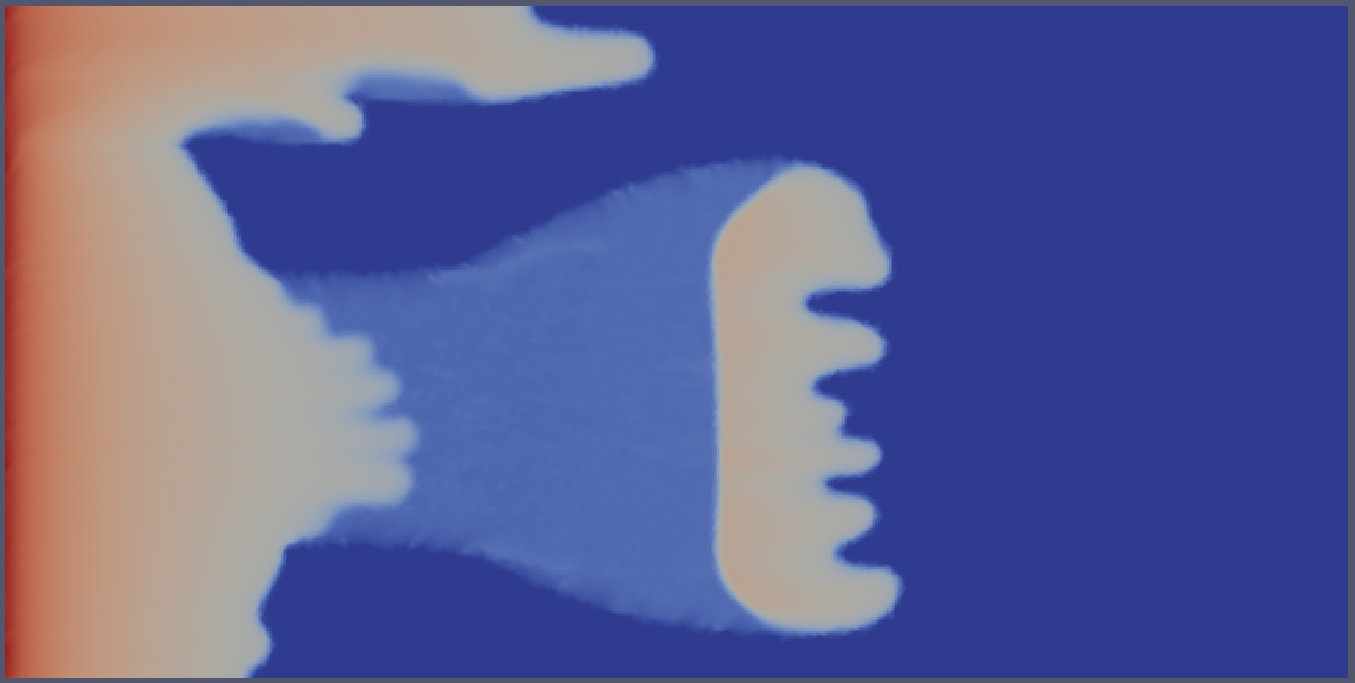
\includegraphics[width=.65\textwidth]{./Pics1/mr10_5regions_fixed/5regions_fixed_500.pdf} 
}
\vspace{0.0cm}
\hbox{\hspace{6.5cm} (a) flow at t=500 (fixed mesh)   
}
\vspace{0.25cm}
\hbox{\hspace{3.5cm}
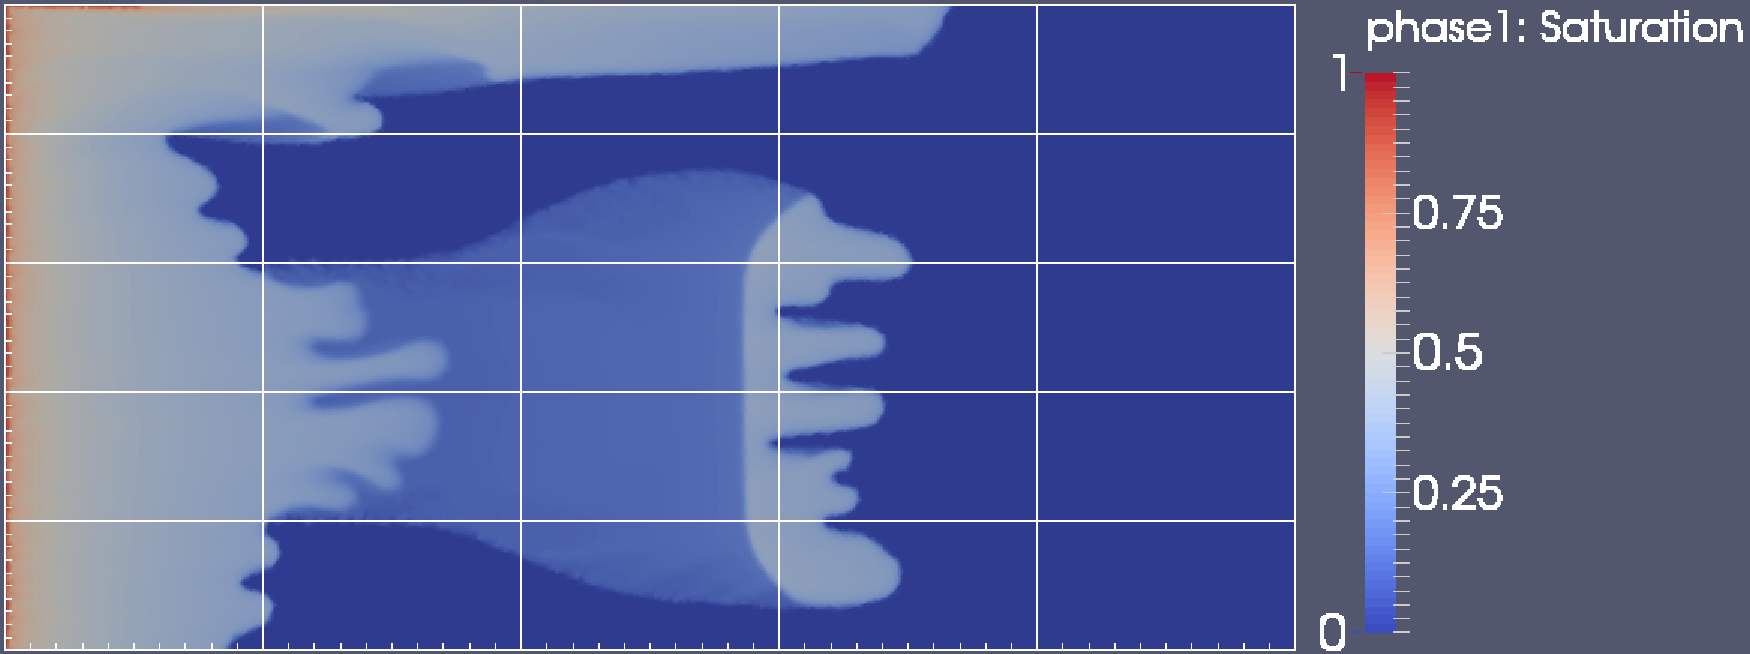
\includegraphics[width=.9\textwidth]{./Pics1/mr10_5regions_adapt/5regions_adapt_500_1.pdf}
}
\vspace{0.0cm}
\hbox{\hspace{6.5cm} (b) flow at t=500 (adaptive mesh)     
}
}     
\caption{At $t=0.25$s ($t=500$, timestemp) cross flow is taking place at the upper part of the formation. The fingers start to becoming more proufound as can been seen at the bottom.}
\label{fig:2testcase_b}
\end{figure}
\end{landscape}
\clearpage



%%%%
%%%%  FIGURE
%%%%
\begin{landscape}
\begin{figure}[ht] 
\vbox{
\hbox{\hspace{3.5cm}
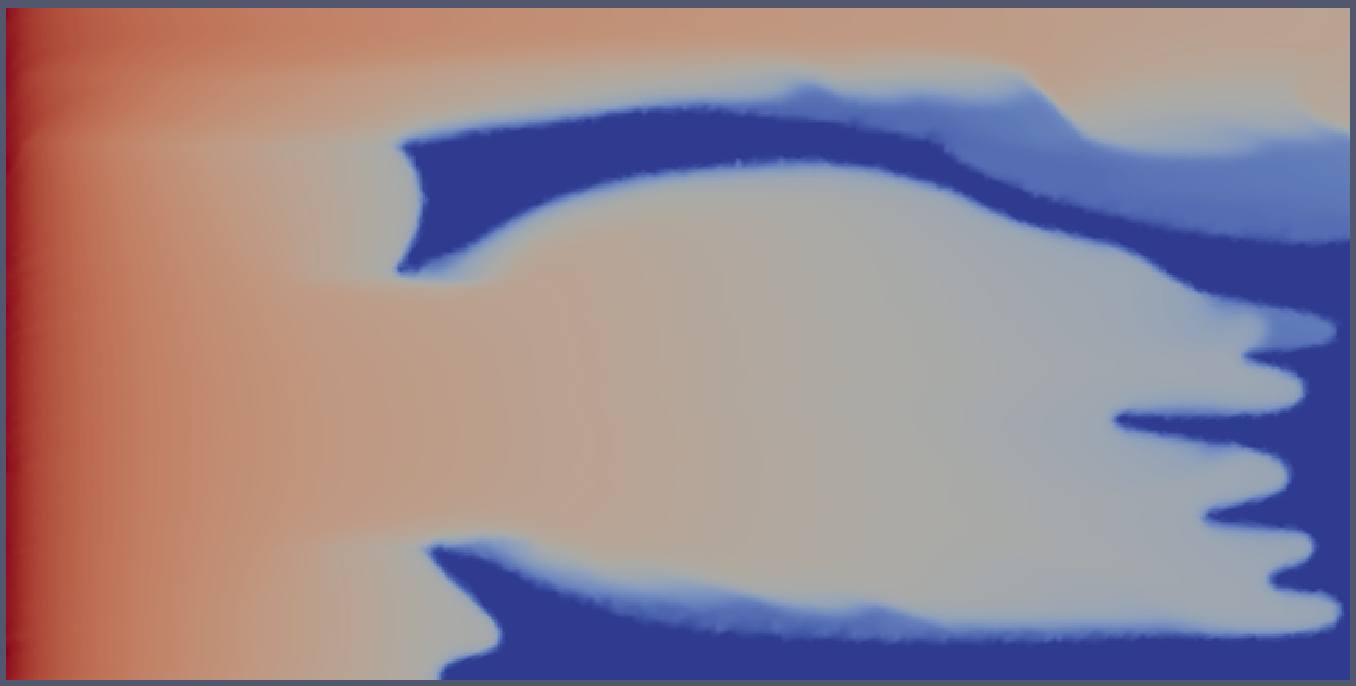
\includegraphics[width=.65\textwidth]{./Pics1/mr10_5regions_fixed/5regions_fixed_1500.pdf} 
}
\vspace{0.0cm}
\hbox{\hspace{6.5cm} (a) flow at t=1500 (fixed mesh)   
}
\vspace{0.25cm}
\hbox{\hspace{3.5cm}
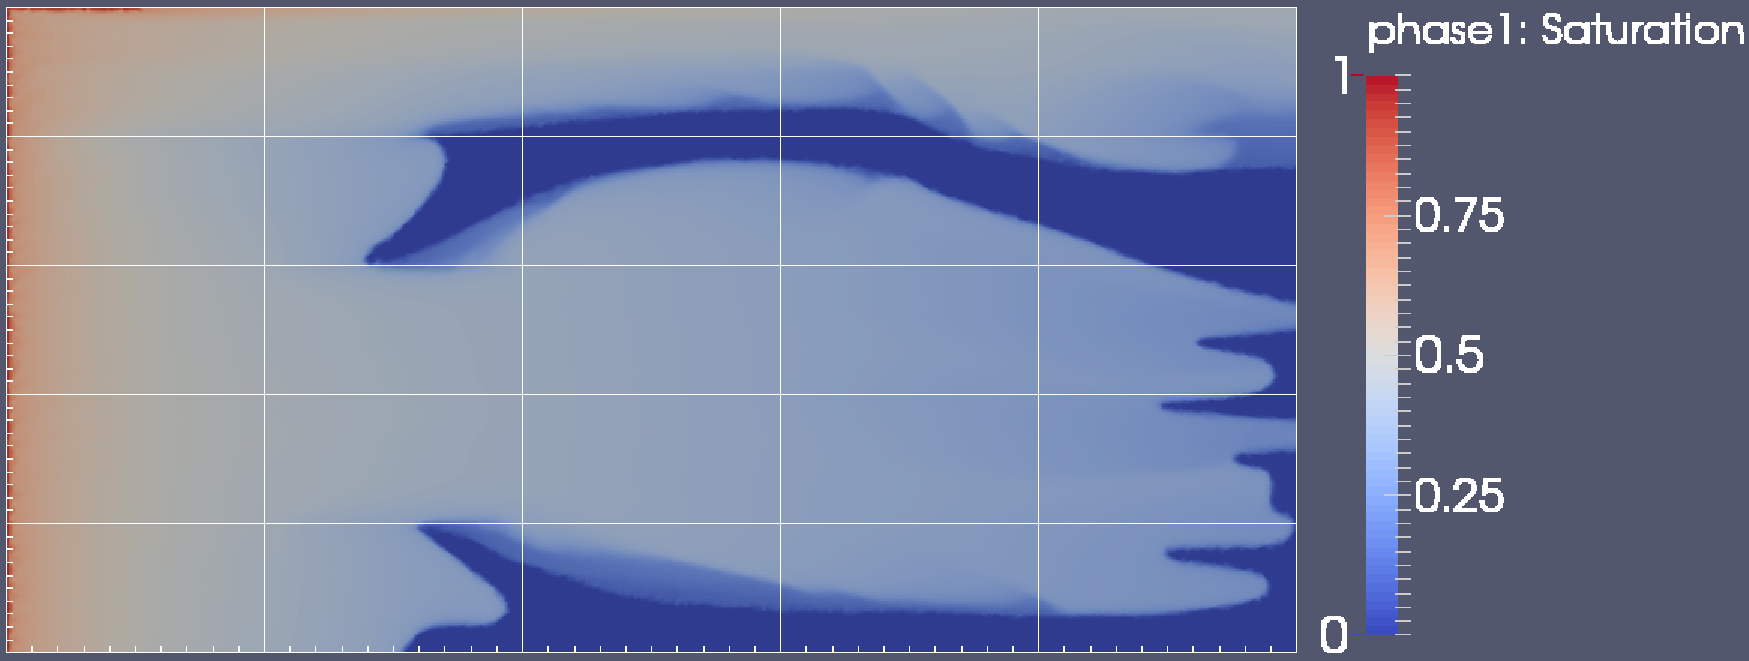
\includegraphics[width=.9\textwidth]{./Pics1/mr10_5regions_adapt/5regions_adapt_1500_1.pdf}
}
\vspace{0.0cm}
\hbox{\hspace{6.5cm} (b) flow at t=1500 (adaptive mesh)     
}
}     
\caption{At $t=0.75 sec$ ($t=1500$, timestemp) the initial cross flow is now fully developed and has travel all the way towards the outlet (right-hand side). and the finger below start forming a front that is also travelling towards the left-hand side.}
\label{fig:2testcase_c}
\end{figure}
\end{landscape}
\clearpage



%%%%
%%%%  FIGURE
%%%%
\begin{landscape}
\begin{figure}[ht] 
\vbox{
\hbox{\hspace{3.5cm}
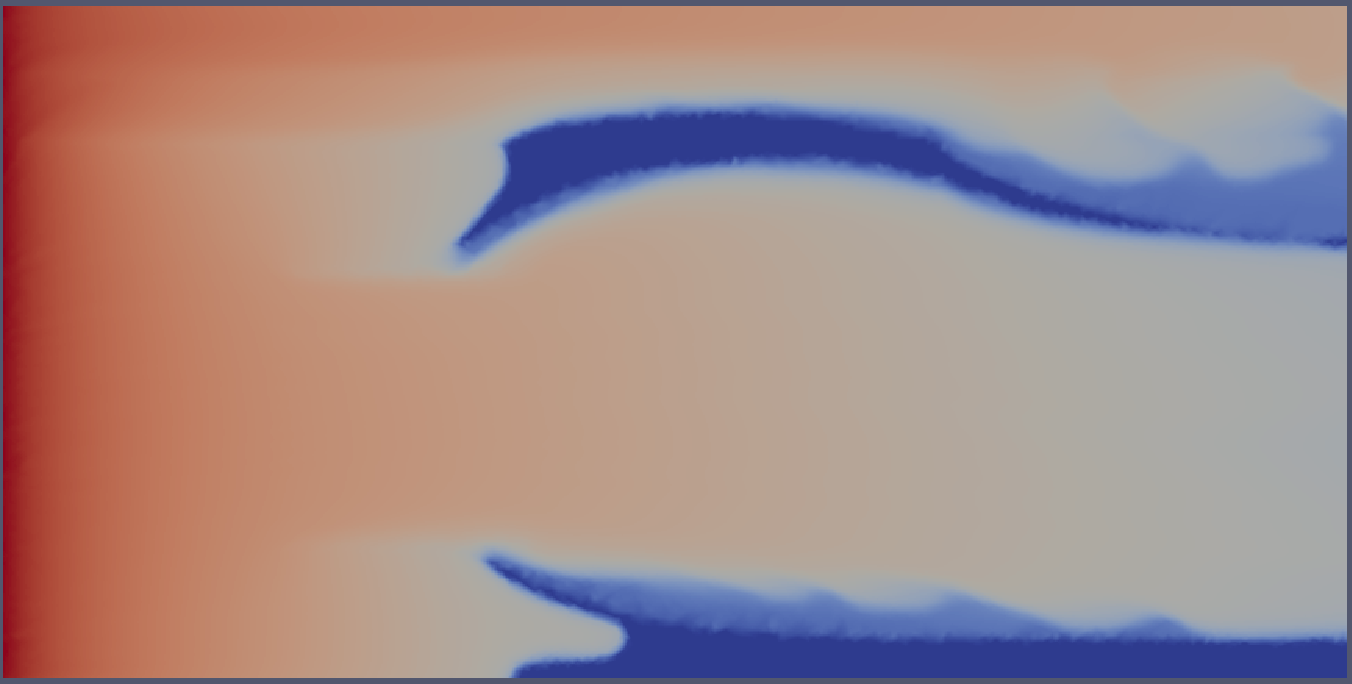
\includegraphics[width=.65\textwidth]{./Pics1/mr10_5regions_fixed/5regions_fixed_2000.pdf} 
}
\vspace{0.0cm}
\hbox{\hspace{6.5cm} (a) flow at t=end (fixed mesh)   
}
\vspace{0.25cm}
\hbox{\hspace{3.5cm}
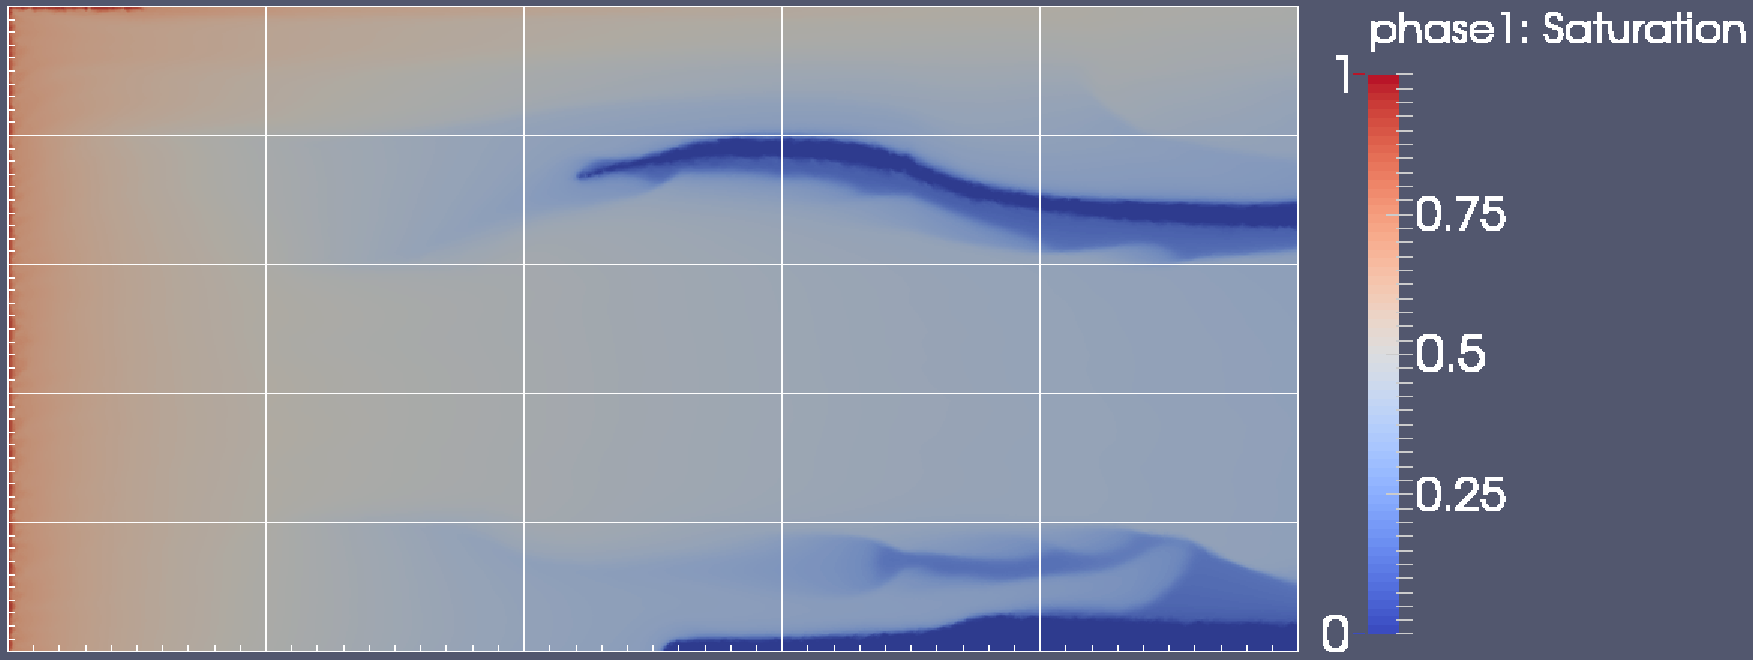
\includegraphics[width=.9\textwidth]{./Pics1/mr10_5regions_adapt/5regions_adapt_3000_1.pdf}
}
\vspace{0.0cm}
\hbox{\hspace{6.5cm} (b) flow at t=end (adaptive mesh)     
}
}     
\caption{Using the $P_{1}DGP_{2}$ element type for VR=$10$ under the same time steps, we compared the impact of fixed and adaptive mesh for the same timeframe. The end of simulation happens at $time=5 sec$ and for the timestemp $t=9999$ while the number of elements in both simulations was approximately $4700$. When adaptive mesh is introduce there is better repersentation of the fluid instabilities as these are developed on time.}
\label{fig:2testcase_d}
\end{figure}
\end{landscape}
\clearpage



%%%%
%%%%  FIGURE
%%%%
\begin{landscape}
\begin{figure}[ht] 
\vbox{
\hbox{\hspace{3.5cm}
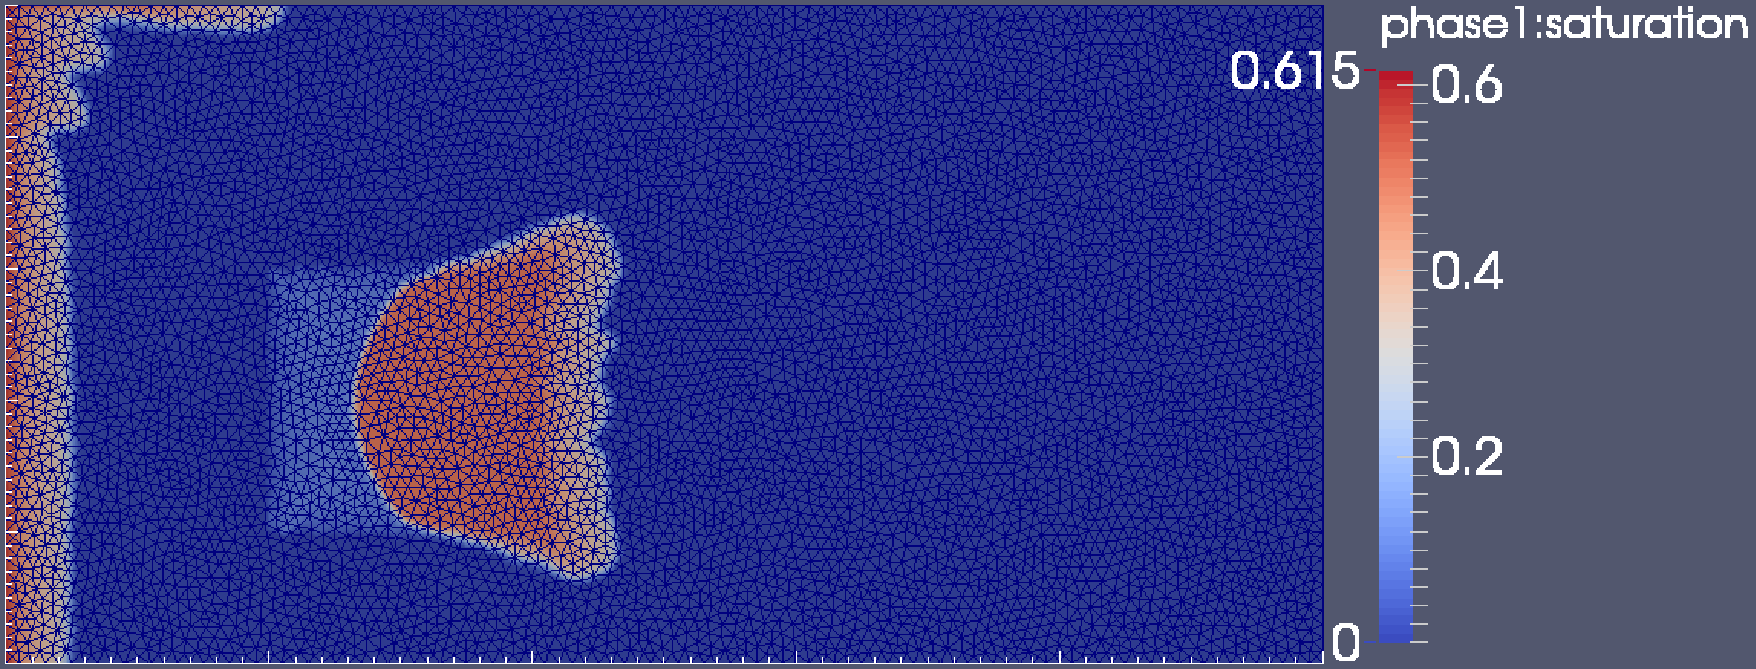
\includegraphics[width=.9\textwidth]{./Pics1/mr10_5regions_fixed_dinlet/5regions_dinlet_fixed_100_1.pdf}
}
\vspace{0.0cm}
\hbox{\hspace{6.5cm} (a) double inlet - fixed mesh   
}
\hbox{\hspace{3.5cm}
  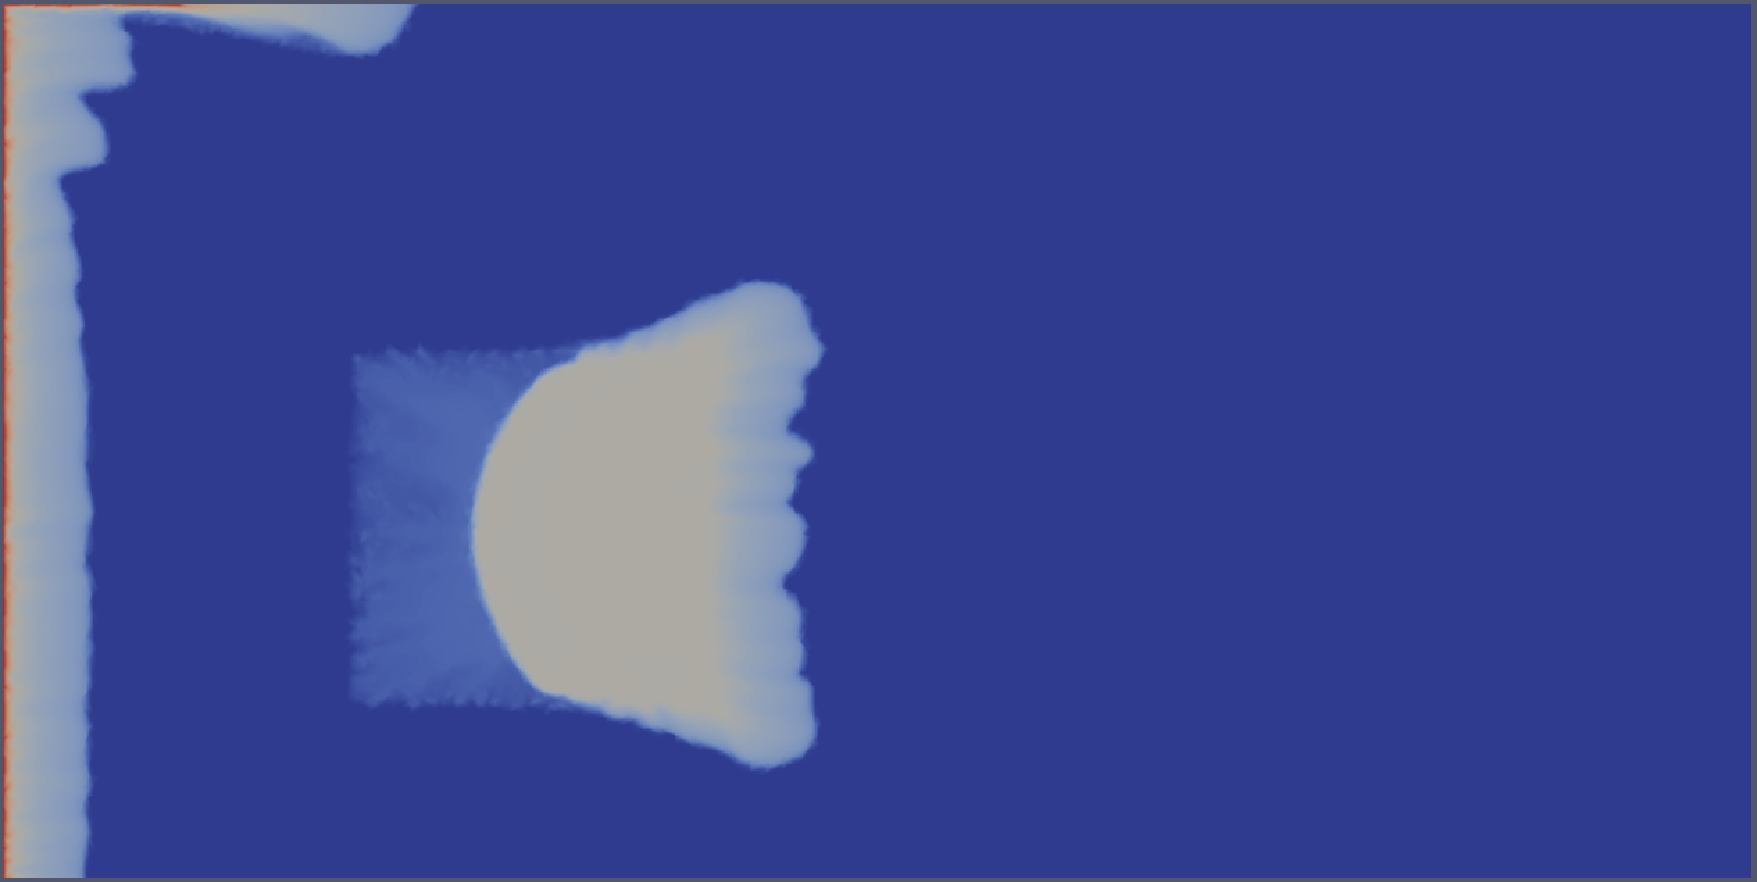
\includegraphics[width=.67\textwidth]{./Pics1/mr10_5regions_adapt_dinlet/5regions_dinlet_adapt_start.pdf}
}
\vspace{0.0cm}
\hbox{\hspace{6.5cm} (b) double inlet adaptive mesh   
}
}     
\caption{Comparing test-cases of fixed and adaptive mesh while a second region/inlet is introduced. For $t=0.101$s, using the $P_{1}DGP_{2}$ element type for MR=$10$ under the same time steps. For this simulation there are $13226$ elements for the fixed messh and $43716$ for the adaptive.}
\label{fig:3testcase_a}
\end{figure}
\end{landscape}
\clearpage

%%%%
%%%%  FIGURE
%%%%
\begin{figure}[ht] 
\vbox{
\hbox{\hspace{3.5cm}
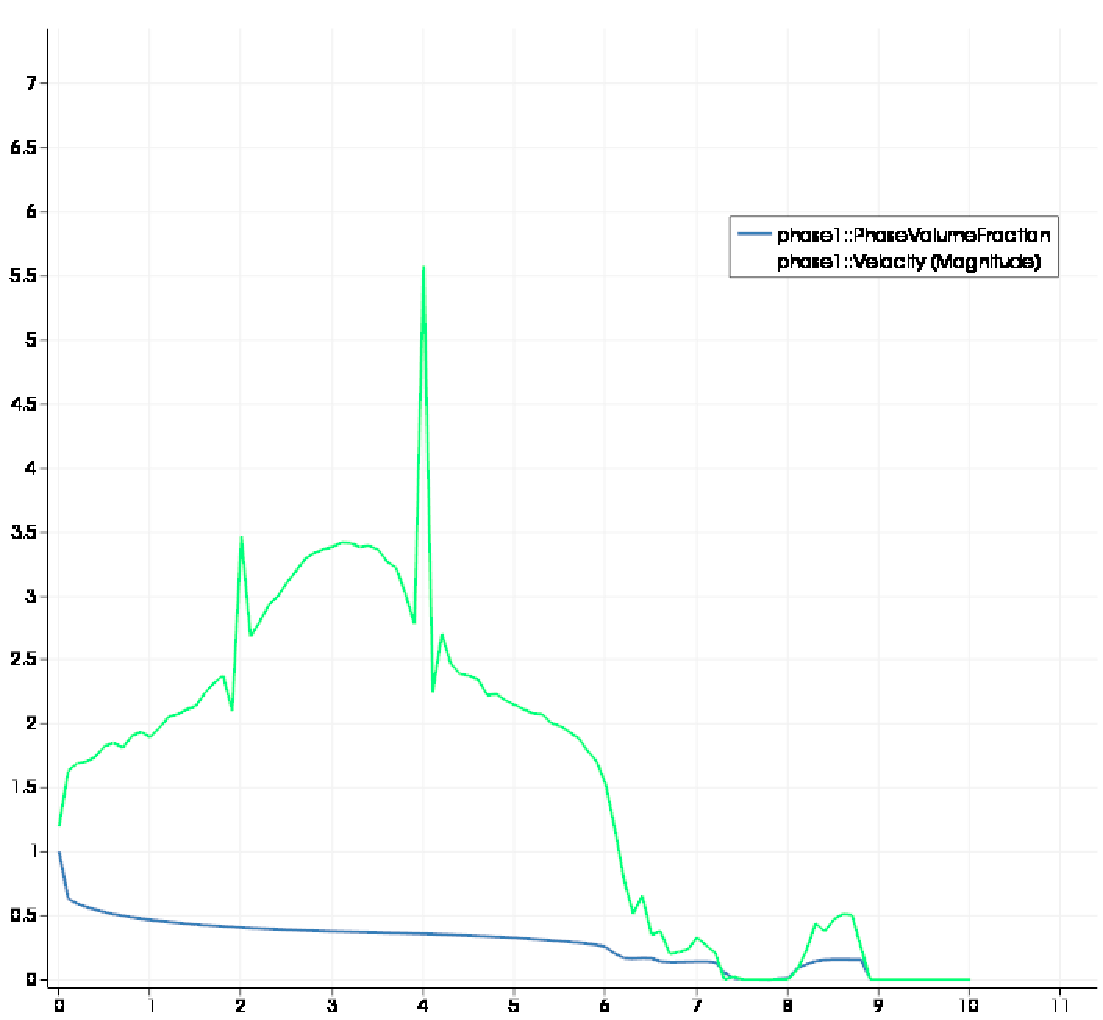
\includegraphics[width=.5\textwidth]{./Pics1/mr10_5regions_adapt/5regions_adapt_vel_magn.pdf} 
}
\vspace{0.0cm}
\hbox{\hspace{5.0cm} (a) single inlet velocity magnitude   
}
\hbox{\hspace{3.5cm}
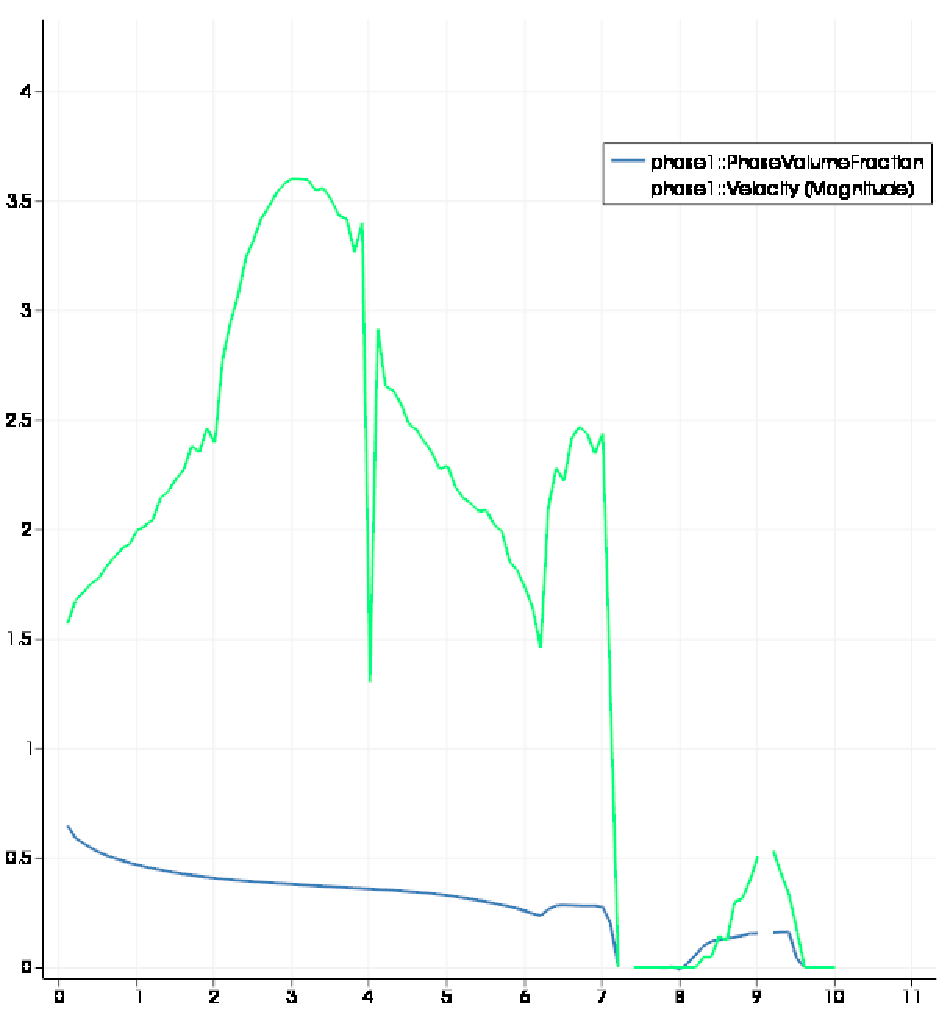
\includegraphics[width=.5\textwidth]{./Pics1/mr10_5regions_adapt_dinlet/5regions_dinlet_adapt_vel_magn.pdf}
}
\vspace{0.0cm}
\hbox{\hspace{5.0cm} (b) double inlet velocity magnitude   
}
}     
\caption{For the same time step, t=1000, these plots describe the velocity magnitudes of the phase $1$ (injected fluid) under the same boundary and initiall conditions. From top to bottom,these graphs describe the velocity magnitude %for fixed mesh is plotted(top), the velocity magnitude 
for adaptive mesh-single inlet (top) and the velocity magnitude for adaptive mesh with double inlet (bottom) as these are also presented in fig.\ref{fig:3testcase_a}. The main difference between the upper and lower plot %is not just the ability to capture in greater detail, the fluid instabilities as they happenduring the finger development and their velocity patterns. While there 
is the impact of the second injection interval as this can be seen from the slope and the rate that the velocity magnitude is changing.}
\label{fig:vel_magn}
\end{figure}

%%%%
%%%%  FIGURE
%%%%
\begin{landscape}
\begin{figure}[ht] 
\vbox{
\hbox{\hspace{3.5cm}
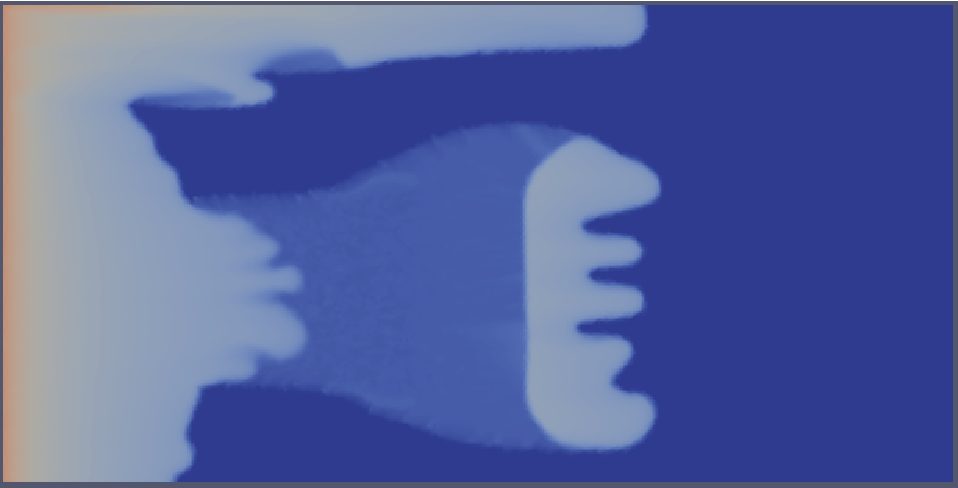
\includegraphics[width=.65\textwidth]{./Pics1/5reg_dinlet_fixed_500.pdf} 
}
\vspace{0.0cm}
\hbox{\hspace{6.5cm} (a) double inlet - fixed mesh   
}
\hbox{\hspace{3.5cm}
\includegraphics[width=.9\textwidth]{./Pics1/5reg_dinlet_adapt_500_1.pdf}
}
\vspace{0.0cm}
\hbox{\hspace{6.5cm} (b) double inlet adaptive mesh   
}
}     
\caption{For $t=5$s there is a comparison between fixed mesh(a) and adaptive mesh(b).}
\label{fig:3testcase_b}
\end{figure}
\end{landscape}
\clearpage

%%%%
%%%%  FIGURE
%%%%
\begin{landscape}
\begin{figure}[ht] 
\vbox{
\hbox{\hspace{3.5cm}
\includegraphics[width=.65\textwidth]{./Pics1/5reg_dinlet_fixed_1500.pdf} 
}
\vspace{0.0cm}
\hbox{\hspace{6.5cm} (a) double inlet - fixed mesh   
}
\hbox{\hspace{3.5cm}
\includegraphics[width=.9\textwidth]{./Pics1/5reg_dinlet_adapt_1500_1.pdf}
}
\vspace{0.0cm}
\hbox{\hspace{6.5cm} (b) double inlet adaptive mesh   
}
}     
\caption{For $t=7.5$s this is a comparison between fixed mesh(a) and adaptive mesh(b).}
\label{fig:3testcase_c}
\end{figure}
\end{landscape}
\clearpage

%%%%
%%%%  FIGURE
%%%%
\begin{landscape}
\begin{figure}[ht] 
\vbox{
\hbox{\hspace{3.5cm}
\includegraphics[width=.65\textwidth]{./Pics1/5reg_dinlet_fixed_end.pdf} 
}
\vspace{0.0cm}
\hbox{\hspace{6.5cm} (a) double inlet - fixed mesh   
}
\hbox{\hspace{3.5cm}
\includegraphics[width=.9\textwidth]{./Pics1/5reg_dinlet_adapt_end_1.pdf}
}
\vspace{0.0cm}
\hbox{\hspace{6.5cm} (b) double inlet adaptive mesh   
}
}     
\caption{This is a comparison between fixed mesh(a) and adaptive mesh(b) at the end of the simulation. For the fixed mesh at this point the maximum number of point is $13226$ while for the adaptive mesh is $7582$ and most of them are located where is needed in the domain.}
\label{fig:3testcase_d}
\end{figure}
\end{landscape}
\clearpage

%%%%
%%%%  FIGURE
%%%%
\begin{landscape}
\begin{figure}[ht] 
\vbox{
\hbox{\hspace{3.5cm}
\includegraphics[width=.8\textwidth]{./Pics1/mr100_fixed/mr100_fixed_500.pdf} 
}
\vspace{0.0cm}
\hbox{\hspace{4.0cm} (a) fixed and unstructured mesh for MR = 100 (start)   
}
\hbox{\hspace{3.5cm}
\includegraphics[width=.8\textwidth]{./Pics1/mr100_fixed/mr100_fixed_1500.pdf}
}
\vspace{0.0cm}
\hbox{\hspace{3.75cm} (b) fixed and unstructured mesh for MR = 100 (t = 1500)   
}
}     
\caption{For the case of VR=$100$ from top to bottom, the number of elements is $4680$ and fixed and unstructured mesh for the same time steps, t=$0.25$ or t=500(a), t=$0.75$ or t=1500(b). }
\label{fig:4testcase_a}
\end{figure}
\end{landscape}
\clearpage

%%%%
%%%%  FIGURE
%%%%
\begin{landscape}
\begin{figure}[ht] 
\vbox{
\hbox{\hspace{3.5cm}
\includegraphics[width=.8\textwidth]{./Pics1/mr100_fixed/mr100_fixed_3000.pdf} 
}
\vspace{0.0cm}
\hbox{\hspace{3.75cm} (c) fixed and unstructured mesh for MR = 100    
}
\hbox{\hspace{3.5cm}
\includegraphics[width=.8\textwidth]{./Pics1/mr100_fixed/mr100_fixed_end.pdf}
}
\vspace{0.0cm}
\hbox{\hspace{7.cm} (d) end of simulations     
}
}     
\caption{screenshot (c) is for t=$1.5$ sec or t=$3000$ and screenshot (d) is for t=$3.175$ sec, at the end of the simulations. }
\label{fig:4testcase_b}
\end{figure}
\end{landscape}
\clearpage



%

%%%
%%%  FIGURE 
%%%
\begin{figure}[h]
\begin{center}
\includegraphics[width=1.\textwidth]{diagrams/bl-exact-meth-upwind.eps}
\end{center}
\caption{Buckley--Leverett test-cases: Saturation solutions for the continuous upwind method for different 1D P$_{1}$DG-P$_{2}$ mesh  resolutions and comparison against standard analytical solution.
\label{bl-exact-meth-upwind}}
\end{figure}

%%%
%%%
%%%  FIGURE 
%%%
\begin{figure}[h]
  %\begin{center}
\vbox{\hbox{\hspace{2.5cm}
    \includegraphics[width=0.62\textwidth]{diagrams/BL_1d_P0DGP1_convergence.eps}}
\vspace{-.0cm}\hbox{\hspace{2.5cm}
    \includegraphics[width=0.62\textwidth]{diagrams/BL_1d_P1DGP2_convergence.eps}}
\vspace{-.0cm}\hbox{\hspace{2.5cm}
    \includegraphics[width=0.62\textwidth]{diagrams/BL_1d_P2DGP3_convergence.eps}}}
   % \includegraphics[width=0.45\textwidth]{BL_2d_P1DGP2_convergence}
    \caption{Buckley--Leverett test-cases: Saturation profiles for a number of element-pairs and numerical resolutions in 1D -- P$_{0}$DG-P$_{1}$ (top), P$_{1}$DG-P$_{2}$ and P$_{2}$DG-P$_{3}$ (bottom).\label{fig:BL_profiles}}
  %\end{center}
\end{figure}

%%%
%%%  FIGURE 
%%%
\begin{figure}[h]
\vbox{\hbox{\hspace{1.cm}
    \includegraphics[width=0.8\textwidth]{diagrams/L1_convergence_rate.eps}}
\vspace{.0cm}\hbox{\hspace{1.cm}
    \includegraphics[width=0.8\textwidth]{diagrams/L2_convergence_rate.eps}}}
    \caption{Buckley--Leverett test-cases: L1 (top) and L2 (bottom) error convergence rates for a number of element pairs. \label{fig:BL_converg-rates}}
\end{figure}

%%%
%%%  FIGURE 
%%%
\begin{figure}[h]
\begin{center}
\includegraphics[width=1.\textwidth]{diagrams/bl-upwind-v-up-and-down.eps}
\end{center}
\caption{Buckley--Leverett test-cases: Comparison of the optimal upwind formulation when using upwinding (OU) and coupled upwind/downwind (OU-D). The finite element interpolation of the saturation field $\left(S_{1}\right)$ is shown at different mesh resolutions. Downwind seems to detract from the accuracy of the solution. \label{bl-upwind-v-up-and-down}}
\end{figure}

%%%
%%%  FIGURE 
%%%
\begin{figure}[h]
\vbox{
\begin{center}
\includegraphics[width=1.\textwidth]{diagrams/bl-exact-meth-cv-0-8-ele50.eps}
\end{center}
\vspace{0.cm}}
\caption{Buckley--Leverett test-cases: Comparison of control volume
  solutions using 80$\%$ upwinding and with optimal upwinding and
  using 50 continuous P$_{1}$DG-P$_{2}$
  elements. \label{bl-exact-meth-cv-0-8-ele50}}
\end{figure}

%%%
%%%  FIGURE 
%%%
\begin{figure}[h]
\begin{center}
\includegraphics[width=1.\textwidth]{diagrams/bl-dg-2eles.eps}
\end{center}
\caption{Buckley--Leverett test-cases: Two element solution using the
  discontinuous formulation. Saturation field from both CV solution
  and FEM interpolation are shown.  \label{bl-dg-2eles}}
\end{figure}

%%%
%%%  FIGURE 
%%%
\begin{figure}[h]
\vbox{
\hbox{\hspace{.3cm}\includegraphics[width=.9\textwidth]{diagrams/bl-dg-4-10-20.eps}}
\vspace{-0.cm}
\hbox{\hspace{.3cm}\includegraphics[width=.9\textwidth]{diagrams/bl-dg-cent-4-10-20.eps}}}
\caption{Buckley--Leverett test-cases: Saturation field obtained from
  the discontinuous and continuous formulation with different mesh
  resolutions. Solutions with (top) and without (bottom) upwinding
  scheme. Notice that oscillations are suppressed with the upwinding
  scheme.\label{bl-dg-cent-4-10-20}}
\end{figure}


%%%
%%%  FIGURE 
%%%
\begin{figure}[h]
\vbox{
\hbox{\hspace{.3cm}\includegraphics[width=.9\textwidth]{diagrams/bl-dg-4-10-vers-cty.eps}}
\vspace{-0.cm}
\hbox{\hspace{.3cm}\includegraphics[width=.9\textwidth]{diagrams/bl-dg-p1-2-4-5-10-20-40.eps}}}
\caption{Buckley--Leverett test-cases: Saturation field obtained from
  (top) continuous and discontinuous (between elements) formulations
  (solution with 50 elements may be considered as a converged
  result). Solution obtained (bottom) from linear pressure (P1)
  formulation with different mesh resolution with comparison against
  P2-pressure formulation (continuous). \label{bl-dg-4-10-vers-cty}}
\end{figure}


%%%
%%%  FIGURE 
%%%
\begin{figure}[H]
\vbox{
\begin{center}
\includegraphics[width=17.5cm,height=12.5cm]{diagrams/bl-dg-4-10-vers-cty}
\end{center}
\vspace{0.cm}}
\caption{Gas saturations shown comparing the accuracy of the
  discontinuous between elements and continuous formulation. The 50
  element continuous solution may be viewed as a converged result.  }
\label{bl-dg-4-10-vers-cty}
\end{figure}

\begin{comment}
%%%
%%%  FIGURE 
%%%
\begin{figure}[h]
\vbox{
\hbox{\hspace{.2cm}
    \includegraphics[width=1.\textwidth]{diagrams/map_2d.png}}
\vspace{1.cm}
\hbox{\hspace{0.2cm}
    \includegraphics[width=1.\textwidth]{./diagrams/map_3d.png}}}
    \caption{Buckley-Leverett test-cases: phase 1 saturation surface maps for a 2- (770 triangles) and 3-D (1207 tetrahedra) simulations (\PN[1]{2} unstructured mesh grids) at time $t=0.5$. \label{fig:maps2d_3d}}
\end{figure}


%%%  FIGURE 
%%%
\begin{figure}[h]
\vbox{\hbox{\hspace{.3cm}
    \includegraphics[width=0.9\textwidth]{diagrams/BL_2d_P1DGP2_convergence.eps}}
\vspace{-.0cm}\hbox{\hspace{.3cm}
    \includegraphics[width=0.9\textwidth]{./diagrams/simulations_2d_3d.eps}}}
    \caption{Buckley-Leverett test-cases: 2- and 3-D phase 1 saturation profiles with \PN[1]{2} elements. Sensitivity analysis for (top) grid resolution using structured \PN[1]{2} mesh, and (bottom) mesh type.\label{fig:BL_2d_profiles}}
\end{figure}

\end{comment}



\end{document}

%%
%% End of tex file.
